\documentclass[12pt,a4paper,oneside]{report}

% ==============================================================================
% GÓI VÀ CẤU HÌNH NGÔN NGỮ, FONT CHỮ
% ==============================================================================
\usepackage[utf8]{inputenc}
\usepackage[vietnamese]{babel}
\usepackage[T5]{fontenc}
\usepackage{mathptmx} % Font Times New Roman chuẩn học thuật

% Cấu hình ký tự unicode cho cây thư mục (nếu có ký tự vẽ khung)
\DeclareUnicodeCharacter{251C}{|--}
\DeclareUnicodeCharacter{2500}{-}
\DeclareUnicodeCharacter{2514}{\`--}
\DeclareUnicodeCharacter{2502}{|}
\DeclareUnicodeCharacter{2014}{--}

% ==============================================================================
% GÓI ĐỊNH DẠNG TRANG & CĂN LỀ CHUẨN ĐỒ ÁN / KHÓA LUẬN
% ==============================================================================
\usepackage{geometry}
\geometry{
    a4paper,
    top=25mm,
    bottom=25mm,
    left=30mm,
    right=20mm,
    headheight=15pt
}
\usepackage{amssymb}

\usepackage{setspace}
\setstretch{1.25} % Giãn dòng chuẩn 1.25 - 1.3
\setlength{\parindent}{1.0cm} % Thụt đầu dòng 1cm
\setlength{\parskip}{4pt}    % Khoảng cách giữa các đoạn

% ==============================================================================
% MÀU SẮC & ĐỒ HỌA
% ==============================================================================
\usepackage{xcolor}
\definecolor{primaryblue}{RGB}{14, 116, 144}   % Xanh chủ đạo (Teal/Cyan đậm)
\definecolor{darknavy}{RGB}{15, 23, 42}       % Xanh navy đậm
\definecolor{codebg}{RGB}{248, 250, 252}      % Màu nền mã nguồn
\definecolor{codeborder}{RGB}{203, 213, 225}  % Viền khối mã nguồn
\definecolor{passgreen}{RGB}{22, 101, 52}     % Màu chữ PASS
\definecolor{passbg}{RGB}{220, 252, 231}      % Màu nền badge PASS

\usepackage{graphicx}
\usepackage{float}
\graphicspath{{images/}{./}{../docs/images/}}

\usepackage{caption}
\captionsetup{
    font=small,
    labelfont=bf,
    labelsep=colon,
    justification=centering,
    skip=6pt
}

% ==============================================================================
% TIÊU ĐỀ CHƯƠNG & MỤC (TITLESEC)
% ==============================================================================
\usepackage{titlesec}

% Định dạng tiêu đề chương: Không xuống dòng vô ích, phong cách hiện đại
\titleformat{\chapter}[block]
  {\normalfont\Large\bfseries\color{darknavy}}
  {\MakeUppercase{CHƯƠNG \thechapter:}}{0.5em}{\MakeUppercase}
\titlespacing*{\chapter}{0pt}{10pt}{14pt}

\titleformat{\section}
  {\normalfont\large\bfseries\color{primaryblue}}
  {\thesection.}{0.5em}{}
\titlespacing*{\section}{0pt}{12pt}{6pt}

\titleformat{\subsection}
  {\normalfont\normalsize\bfseries\color{darknavy}}
  {\thesubsection.}{0.5em}{}
\titlespacing*{\subsection}{0pt}{10pt}{4pt}

\titleformat{\subsubsection}
  {\normalfont\normalsize\bfseries\itshape}
  {\thesubsubsection.}{0.5em}{}
\titlespacing*{\subsubsection}{0pt}{8pt}{4pt}

% ==============================================================================
% HEADER & FOOTER (FANCYHDR)
% ==============================================================================
\usepackage{fancyhdr}
\pagestyle{fancy}
\fancyhf{}
\fancyhead[L]{\small\textit{Hệ thống Quản lý Kho hàng -- Báo cáo Bài tập lớn}}
\fancyhead[R]{\small\textit{ICTU -- Khoa CNTT}}
\fancyfoot[C]{\thepage}
\renewcommand{\headrulewidth}{0.4pt}
\renewcommand{\footrulewidth}{0.4pt}

% ==============================================================================
% BẢNG BIỂU & DANH SÁCH & TIKZ
% ==============================================================================
\usepackage{tabularx}
\usepackage{booktabs}
\usepackage{colortbl}
\usepackage{array}
\usepackage{enumitem}
\setlist{nosep, leftmargin=1.5cm} % Danh sách gọn gàng

\usepackage{tikz}
\usetikzlibrary{calc}
\usepackage{tcolorbox}
\tcbuselibrary{skins,breakable}

\usepackage{dirtree}
\renewcommand*\DTstyle{\ttfamily\small}

% ==============================================================================
% MÃ NGUỒN & LIÊN KẾT HYPERREF
% ==============================================================================
\usepackage{listings}
\lstset{
    backgroundcolor=\color{codebg},
    basicstyle=\ttfamily\footnotesize,
    breaklines=true,
    breakatwhitespace=false,
    frame=single,
    rulecolor=\color{codeborder},
    numbers=none,
    showstringspaces=false,
    tabsize=2,
    keepspaces=true
}

\usepackage{hyperref}
\hypersetup{
    colorlinks=true,
    linkcolor=darknavy,
    citecolor=primaryblue,
    urlcolor=primaryblue,
    pdftitle={BÁO CÁO BÀI TẬP LỚN - HỆ THỐNG QUẢN LÝ KHO HÀNG (ICTU)},
    pdfauthor={Thân Phú Cường},
    pdfsubject={DevOps - Triển khai và Quản trị Hệ thống}
}

% Lệnh tạo badge PASS
\newcommand{\badgepass}{\colorbox{passbg}{\textcolor{passgreen}{\textbf{PASS}}}}

% ==============================================================================
% BẮT ĐẦU TÀI LIỆU
% ==============================================================================
\begin{document}

% ------------------------------------------------------------------------------
% TRANG BÌA (ACADEMIC COVER PAGE VỚI KHUNG KÉP TIKZ)
% ------------------------------------------------------------------------------
\begin{titlepage}
\thispagestyle{empty}
\begin{tikzpicture}[remember picture, overlay]
  % Khung viền ngoài đậm
  \draw[line width = 2pt, color=darknavy] 
    ($(current page.north west) + (22mm,-18mm)$) 
    rectangle 
    ($(current page.south east) + (-15mm,18mm)$);
  % Khung viền trong mảnh
  \draw[line width = 0.8pt, color=darknavy] 
    ($(current page.north west) + (23.5mm,-19.5mm)$) 
    rectangle 
    ($(current page.south east) + (-16.5mm,19.5mm)$);
\end{tikzpicture}

\begin{center}
    {\fontsize{13pt}{16pt}\selectfont \textbf{ĐẠI HỌC THÁI NGUYÊN}}\\[4pt]
    {\fontsize{14pt}{17pt}\selectfont \textbf{TRƯỜNG ĐẠI HỌC CÔNG NGHỆ THÔNG TIN VÀ TRUYỀN THÔNG}}\\[3pt]
    {\fontsize{13pt}{16pt}\selectfont \textbf{KHOA CÔNG NGHỆ THÔNG TIN}}\\[6pt]
    {\color{primaryblue}\rule{0.6\linewidth}{1.2pt}}\\[2pt]
    {\color{darknavy}$\bigstar$\quad$\bigstar$\quad$\bigstar$}\\[14pt]

    % Logo trường ICTU
    
\includegraphics[width=3.4cm]{images/ictu_logo.png}\\[16pt]

    {\fontsize{14pt}{18pt}\selectfont \textbf{BÁO CÁO BÀI TẬP LỚN}}\\[6pt]
    {\fontsize{12pt}{15pt}\selectfont \textbf{HỌC PHẦN: TRIỂN KHAI \& QUẢN TRỊ HỆ THỐNG / DEVOPS}}\\[14pt]

    % Tên đề tài
    {\fontsize{16pt}{22pt}\selectfont \textbf{\color{primaryblue}XÂY DỰNG VÀ TRIỂN KHAI HỆ THỐNG\\QUẢN LÝ KHO HÀNG}}\\[4pt]
    {\fontsize{14pt}{18pt}\selectfont \textbf{\color{darknavy}(INVENTORY MANAGEMENT SYSTEM)}}\\[12pt]

    {\fontsize{12pt}{15pt}\selectfont \textbf{ĐỀ TÀI: ĐỀ SỐ 05} \quad|\quad \textbf{Ngành: Công nghệ thông tin}}\\[22pt]

    % Khung thông tin Sinh viên & Giảng viên
    \vspace*{\fill}
    \begin{tcolorbox}[
        enhanced,
        colback=white,
        colframe=codeborder,
        arc=3mm,
        width=0.92\linewidth,
        boxrule=1pt
    ]
    \renewcommand{\arraystretch}{1.35}
    \begin{tabularx}{\linewidth}{lX lX}
        \multicolumn{2}{l}{\textbf{\color{primaryblue}SINH VIÊN THỰC HIỆN:}} & \multicolumn{2}{l}{\textbf{\color{primaryblue}GIẢNG VIÊN HƯỚNG DẪN:}} \\
        Họ và tên: & \textbf{Thân Phú Cường} & Giảng viên: & \textbf{TS. Vũ Văn Diện} \\
        MSSV: & \textbf{DTC245200356} & Môn học: & \textbf{Triển khai \& Quản trị Hệ thống} \\
        Lớp: & \textbf{CNTTK23L} & Khoa: & \textbf{Công nghệ thông tin} \\
    \end{tabularx}
    \end{tcolorbox}
    \vspace*{\fill}

    {\fontsize{12pt}{15pt}\selectfont \textbf{THÁI NGUYÊN, NĂM 2026}}
\end{center}
\end{titlepage}

% ------------------------------------------------------------------------------
% LỜI CẢM ƠN (ACKNOWLEDGEMENT)
% ------------------------------------------------------------------------------
\newpage
\pagenumbering{roman}
\setcounter{page}{1}

\begin{center}
    {\fontsize{16pt}{20pt}\selectfont \textbf{\color{primaryblue}LỜI CẢM ƠN}}
\end{center}
\vspace{10pt}

Em xin gửi lời cảm ơn chân thành và sâu sắc nhất đến \textbf{thầy TS. Vũ Văn Diện}, giảng viên môn học \textit{Triển khai \& Quản trị Hệ thống}, người đã tận tình truyền đạt những kiến thức quý báu, định hướng phương pháp tư duy kỹ thuật và hỗ trợ chúng em trong suốt quá trình hoàn thành bài tập lớn với đề tài: \textbf{''Xây dựng và Triển khai Hệ thống Quản lý Kho hàng (Inventory Management System)''}.

Những bài giảng chuyên sâu của thầy về kiến trúc ảo hóa container, cổng điều hướng Gateway Nginx, giải pháp giám sát chỉ số thời gian thực Prometheus -- Grafana và hệ thống truy vết log tập trung Loki -- Promtail đã giúp em không chỉ nắm vững lý thuyết mà còn tự tin vận dụng vào xây dựng một hạ tầng dịch vụ chuẩn mực DevOps.

Dù đã dành nhiều nỗ lực và tâm huyết để hoàn thiện đồ án một cách chỉn chu nhất, song do giới hạn về kiến thức và kinh nghiệm thực tiễn, bản báo cáo khó tránh khỏi những thiếu sót nhất định. Em rất mong tiếp tục nhận được những nhận xét, góp ý quý báu từ thầy để hệ thống ngày càng được hoàn thiện và nâng cao hơn nữa.

Kính chúc thầy luôn dồi dào sức khỏe, hạnh phúc và gặt hái được nhiều thành tựu rực rỡ trong sự nghiệp nghiên cứu và giảng dạy!

\vspace{25pt}
\begin{flushright}
    \textit{Thái Nguyên, ngày 20 tháng 10 năm 2026}\\[6pt]
    \textbf{Sinh viên thực hiện}\\[30pt]
    \textbf{Thân Phú Cường}
\end{flushright}

% ------------------------------------------------------------------------------
% MỤC LỤC & DANH MỤC HÌNH VẼ, BẢNG BIỂU
% ------------------------------------------------------------------------------
\newpage
\tableofcontents

\newpage
\listoffigures
\vspace{15pt}
\listoftables

% ==============================================================================
% NỘI DUNG CHÍNH (PAGENUMBERING ARABIC)
% ==============================================================================
\newpage
\pagenumbering{arabic}
\setcounter{page}{1}

% ------------------------------------------------------------------------------
% CHƯƠNG 1: MỞ ĐẦU & TỔNG QUAN HỆ THỐNG
% ------------------------------------------------------------------------------
\chapter{Mở đầu \& Tổng quan Hệ thống}

\section{Đặt vấn đề \& Mục tiêu Đề tài}
Trong bối cảnh chuyển đổi số toàn diện và sự bùng nổ của các ứng dụng thương mại điện tử, dịch vụ chuỗi cung ứng logistics hiện đại, khối lượng giao dịch và tần suất luân chuyển hàng hóa tại các doanh nghiệp ngày càng tăng trưởng với tốc độ cấp số nhân. Với các phương pháp quản lý kho thủ công truyền thống qua sổ sách hoặc các file tính rời rạc thiếu đồng bộ, bộ phận vận hành kho liên tục đối mặt với những thách thức nghiêm trọng:
\begin{itemize}
    \item Sai lệch số liệu tồn kho giữa thực tế và ghi nhận sổ sách.
    \item Chậm trễ trong điều phối hàng hóa, thiếu cơ chế cảnh báo chủ động khi hàng hóa chạm ngưỡng an toàn.
    \item Không kiểm soát chặt chẽ trách nhiệm luân chuyển giữa các nhân viên trong từng ca làm việc.
    \item Thiếu cơ chế theo dõi trạng thái tải tài nguyên máy chủ và truy vết sự cố hệ thống theo thời gian thực.
\end{itemize}

Xuất phát từ yêu cầu thực tế đó, mục tiêu của đề tài không chỉ dừng lại ở việc phát triển ứng dụng Web Quản lý Kho hàng đáp ứng trọn vẹn nghiệp vụ nghiệp vụ nhập -- xuất -- tồn mà còn triển khai đồng bộ theo mô hình \textbf{Chuẩn vận hành hệ thống hiện đại (DevOps / SRE / Containerization)}:
\begin{enumerate}
    \item \textbf{Containerization:} Đóng gói độc lập toàn bộ các dịch vụ ứng dụng, cơ sở dữ liệu và công cụ quản trị bằng Docker và điều phối qua Docker Compose.
    \item \textbf{Cổng bảo mật Gateway (Reverse Proxy):} Cấu hình Nginx đóng vai trò điểm chạm duy nhất, tiếp nhận lưu lượng mạng, chuyển hướng tự động HTTP sang HTTPS với chứng chỉ SSL/TLS tự ký, đồng thời thiết lập đầy đủ 5 tiêu chuẩn HTTP Security Headers.
    \item \textbf{Giám sát Toàn diện (Monitoring):} Tích hợp bộ đôi Prometheus và Grafana, tự động nạp cấu hình DataSource và Dashboards giám sát tài nguyên máy chủ và cơ sở dữ liệu MySQL theo thời gian thực.
    \item \textbf{Quản lý Log Tập trung (Centralized Logging):} Ứng dụng giải pháp Grafana Loki kết hợp Promtail để thu thập log thời gian thực từ Nginx và Web App, thực thi 3 câu truy vấn LogQL chuyên sâu phục vụ cảnh báo và khắc phục sự cố.
    \item \textbf{Gia cố An toàn (Hardening):} Tuân thủ nghiêm ngặt các nguyên tắc bảo mật: Non-root user trong container, phân vùng mạng Docker Networks độc lập, cô lập cổng CSDL MySQL, bảo vệ biến môi trường và giới hạn tài nguyên CPU/RAM.
\end{enumerate}

\section{Kiến trúc Tổng thể Hệ thống}
Hệ thống được thiết kế theo mô hình kiến trúc phân tầng dịch vụ chuẩn mực (Multi-tier Architecture), đảm bảo tính cô lập, khả năng mở rộng linh hoạt và an toàn dữ liệu:
\begin{enumerate}
    \item \textbf{Tầng 1 -- User / Client Layer:} Người dùng truy cập hệ thống thông qua các trình duyệt web bảo mật (Chrome, Edge, Firefox) thông qua giao thức HTTP/HTTPS.
    \item \textbf{Tầng 2 -- Reverse Proxy Gateway Layer:} Cụm Nginx tiếp nhận các kết nối mạng bên ngoài tại cổng 80 và 443. Nginx đảm nhiệm nhiệm vụ ép buộc chuyển hướng toàn bộ lưu lượng HTTP sang HTTPS bằng mã phản hồi \texttt{301 Moved Permanently}, giải mã SSL/TLS, gán các HTTP Security Headers phòng thủ và định tuyến thông minh:
    \begin{itemize}
        \item Đường dẫn \texttt{/} chuyển tiếp lưu lượng vào Web Application (PHP).
        \item Đường dẫn \texttt{/pma/} định tuyến vào cổng quản trị cơ sở dữ liệu phpMyAdmin.
        \item Đường dẫn \texttt{/grafana/} chuyển tiếp tới trung tâm giám sát Grafana.
    \end{itemize}
    \item \textbf{Tầng 3 -- Application \& Storage Layer:}
    \begin{itemize}
        \item \textit{Web Application (PHP 8.2 / Apache):} Xử lý toàn bộ logic kho hàng (quản lý sản phẩm, danh mục, nhà cung cấp, nhập xuất kho, in ấn phiếu và xuất báo cáo).
        \item \textit{Database (MySQL 8.0):} Hệ quản trị CSDL quan hệ lưu trữ dữ liệu kho, đảm bảo tính toàn vẹn dữ liệu theo tiêu chuẩn giao dịch ACID.
        \item \textit{phpMyAdmin:} Giao diện trực quan hỗ trợ quản trị viên thao tác trực tiếp với CSDL an toàn.
    \end{itemize}
    \item \textbf{Tầng 4 -- Monitoring \& Centralized Logging Layer:}
    \begin{itemize}
        \item \textit{Prometheus:} Máy chủ kéo chỉ số (Pull model) thu thập metrics định kỳ từ Node Exporter (tài nguyên host), MySQL Exporter (hiệu năng CSDL) và cAdvisor (tài nguyên container).
        \item \textit{Grafana:} Trung tâm trực quan hóa các chỉ số hiệu năng và dòng nhật ký lên các bảng điều khiển trực quan.
        \item \textit{Promtail:} Agent thu gom tệp log từ Nginx (\texttt{/var/log/nginx/}) và Web App (\texttt{/var/log/app/app.log}), gắn nhãn metadata và đẩy về Loki qua API.
        \item \textit{Loki:} Hệ thống lưu trữ và đánh chỉ mục nhật ký tập trung, phục vụ truy vấn LogQL tốc độ cao.
    \end{itemize}
\end{enumerate}

% ------------------------------------------------------------------------------
% CHƯƠNG 2: CẤU TRÚC MÃ NGUỒN & QUẢN LÝ TRÊN GITHUB
% ------------------------------------------------------------------------------
\chapter{Cấu trúc Mã nguồn \& Quản lý trên GitHub}

\section{Quy chuẩn Quản lý Mã nguồn}
Toàn bộ mã nguồn ứng dụng Web Quản lý kho, các tệp cấu hình hạ tầng Docker Compose, Nginx, Prometheus, Loki, Promtail và tài liệu kiểm thử được quản lý tập trung trên GitHub tuân thủ quy trình Git Workflow chuyên nghiệp:
\begin{itemize}
    \item \textbf{Tài khoản GitHub \& Repository:} Repository được khởi tạo với tên theo chuẩn Mã số Sinh viên: \href{https://github.com/cuongcoder123/DTC245200356-QLKH}{\texttt{cuongcoder123/DTC245200356-QLKH}}.
    \item \textbf{Quy trình Git Commit:} Mỗi giai đoạn triển khai tương ứng với các commit rõ ràng, ghi chú chi tiết công việc hoàn thành và tuần tự theo yêu cầu đề bài (Commit 1: Nginx SSL \& Headers, Commit 2: Prometheus \& Grafana, Commit 3: Loki \& Promtail).
\end{itemize}

\section{Cấu trúc Thư mục Dự án}
Dự án được tổ chức khoa học với cấu trúc phân tách rõ ràng giữa mã nguồn ứng dụng nghiệp vụ và các tệp cấu hình dịch vụ hạ tầng:

\begin{tcolorbox}[
    enhanced,
    colback=codebg,
    colframe=codeborder,
    arc=2mm,
    title=\textbf{\color{darknavy}Sơ đồ Cây Thư mục Hệ thống},
    fonttitle=\small\bfseries
]
\dirtree{%
.1 \textbf{DTC245200356-QLKH/}.
.2 docker-compose.yml.
.2 .env.example.
.2 README.md.
.2 nginx/.
.3 nginx.conf.
.3 conf.d/.
.4 default.conf.
.3 ssl/.
.4 server.crt.
.4 server.key.
.2 app/.
.3 src/ \dots{} \textit{\textsf{(Mã nguồn Website Quản lý kho: PHP/Apache)}}.
.3 Dockerfile.
.2 prometheus/.
.3 prometheus.yml.
.2 promtail/.
.3 promtail-config.yml.
.2 loki/.
.3 loki-config.yml.
.2 grafana/.
.3 provisioning/.
.4 datasources/.
.4 dashboards/.
}
\end{tcolorbox}

\begin{table}[H]
\centering
\small
\renewcommand{\arraystretch}{1.25}
\begin{tabularx}{\linewidth}{|l|X|}
\hline
\rowcolor{codebg}
\textbf{Thành phần / Thư mục} & \textbf{Vai trò và Chức năng trong Hệ thống} \\
\hline
\texttt{docker-compose.yml} & Tệp điều phối trung tâm khởi chạy đồng bộ cụm 10 container dịch vụ. \\
\hline
\texttt{.env.example} & Tệp mẫu khai báo biến môi trường an toàn (được đưa vào \texttt{.gitignore}). \\
\hline
\texttt{README.md} & Cẩm nang hướng dẫn cài đặt, kiến trúc tổng thể và kiểm thử hệ thống. \\
\hline
\texttt{nginx/} & Cổng Gateway Reverse Proxy, chứng chỉ SSL tự ký và 5 tiêu chuẩn Security Headers. \\
\hline
\texttt{app/} & Mã nguồn Web Quản lý kho (PHP 8.2), Dockerfile đóng gói với Non-root user (\texttt{appuser}). \\
\hline
\texttt{prometheus/} & Cấu hình Scrape Metrics định kỳ 15s thu thập từ Node Exporter và MySQL Exporter. \\
\hline
\texttt{promtail/} & Thu gom log tệp từ Nginx và Web App, gắn nhãn định danh chuyển tiếp về Loki. \\
\hline
\texttt{loki/} & Kho lưu trữ và đánh chỉ mục nhật ký tập trung phục vụ các truy vấn LogQL. \\
\hline
\texttt{grafana/} & Tự động nạp sẵn (Provisioning) DataSource và các Dashboards giám sát trực quan. \\
\hline
\end{tabularx}
\caption{Mô tả Chi tiết Các Thành phần trong Cấu trúc Thư mục Dự án}
\label{tab:project_structure}
\end{table}

\section{Nội dung Hướng dẫn README.md}
Tệp \texttt{README.md} tại thư mục gốc repository đóng vai trò cẩm nang hướng dẫn vận hành toàn diện cho đội ngũ kỹ sư và giảng viên thẩm định. Tài liệu cung cấp đầy đủ:
\begin{itemize}
    \item Bảng tổng hợp cổng dịch vụ (Port Mapping) và đường dẫn truy cập qua Nginx Gateway.
    \item Hướng dẫn khởi chạy toàn bộ 10 container chỉ với một câu lệnh:
    \begin{lstlisting}[language=bash]
docker-compose up -d --build
    \end{lstlisting}
    \item Hướng dẫn kiểm tra trạng thái hoạt động của các tiến trình container:
    \begin{lstlisting}[language=bash]
docker-compose ps
    \end{lstlisting}
    \item Danh sách tài khoản đăng nhập mặc định cho các dịch vụ (Web App, phpMyAdmin, Grafana) và danh mục kiểm thử thực nghiệm.
\end{itemize}

% ------------------------------------------------------------------------------
% CHƯƠNG 3: TRIỂN KHAI WEBSITE & CƠ SỞ DỮ LIỆU MYSQL
% ------------------------------------------------------------------------------
\chapter{Triển khai Website Quản lý Kho \& CSDL MySQL}

\section{Thiết kế Cơ sở Dữ liệu MySQL 8.0}
Cơ sở dữ liệu \texttt{inventory\_db} được thiết kế chuẩn hóa bậc 3 (3NF) gồm 6 bảng thực thể quan hệ chặt chẽ:
\begin{enumerate}
    \item \texttt{users}: Quản lý danh sách tài khoản người dùng, băm mật khẩu với thuật toán \texttt{BCRYPT}, phân quyền theo vai trò (\texttt{admin} -- Quản trị viên toàn quyền, \texttt{staff} -- Thủ kho phụ trách nhập xuất).
    \item \texttt{categories}: Quản lý các nhóm danh mục phân loại mặt hàng trong kho (Linh kiện máy tính, Thiết bị mạng, Thiết bị ngoại vi, Phụ kiện, Thiết bị lưu trữ).
    \item \texttt{suppliers}: Lưu trữ hồ sơ các nhà cung cấp đối tác chiến lược (tên doanh nghiệp, mã số thuế, hotline, email liên hệ và địa chỉ trụ sở).
    \item \texttt{products}: Quản lý chi tiết từng SKU sản phẩm: mã hàng, danh mục trực thuộc, đơn vị tính, giá nhập dự toán, giá bán niêm yết, số lượng tồn kho thực tế và ngưỡng tồn kho tối thiểu (\texttt{min\_stock}).
    \item \texttt{inventory\_transactions}: Lưu vết toàn bộ lịch sử các giao dịch biến động kho hàng (Nhập kho -- \texttt{IMPORT}, Xuất kho -- \texttt{EXPORT}), mã phiếu, người phụ trách, đối tác và ghi chú nghiệp vụ.
    \item \texttt{system\_logs}: Lưu nhật ký hoạt động hệ thống nội bộ, phục vụ kiểm toán bảo mật và đối soát chéo dữ liệu.
\end{enumerate}

\section{Chức năng Nghiệp vụ \& Giao diện Website Quản lý Kho}

\subsection{Giao diện Đăng nhập Hệ thống (Authentication \& RBAC)}
Hệ thống sử dụng cơ chế xác thực phiên an toàn: mật khẩu người dùng được băm một chiều với thuật toán \texttt{BCRYPT}. Phiên đăng nhập được quản lý an toàn bằng Session Cookie với cờ bảo vệ \texttt{HttpOnly} và \texttt{SameSite=Lax}, giúp ngăn ngừa triệt để nguy cơ đánh cắp phiên qua tấn công XSS hoặc CSRF. Giao diện đăng nhập hỗ trợ hiển thị thông báo lỗi bảo mật tức thì khi phát hiện thông tin không chính xác.

\begin{figure}[H]
    \centering
    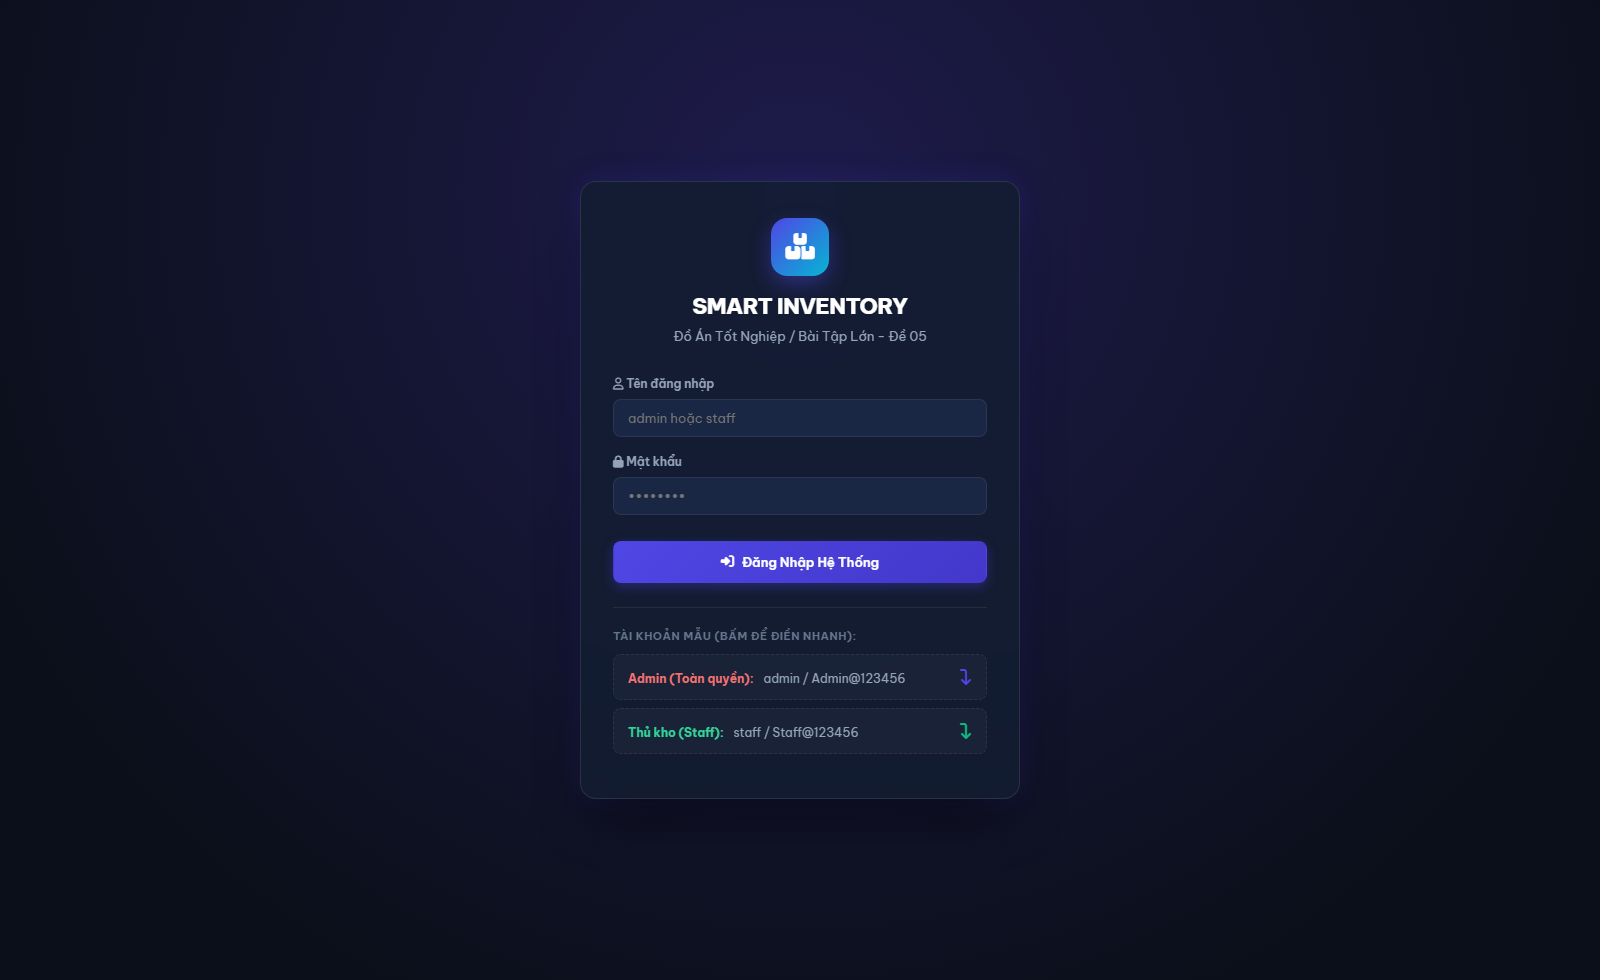
\includegraphics[width=0.92\linewidth]{images/01_dang_nhap.png}
    \caption{Giao diện Đăng nhập An toàn Hệ thống}
    \label{fig:login}
\end{figure}

\subsection{Bảng Điều khiển Tổng quan (Dashboard Quản lý Kho)}
Dashboard đóng vai trò trung tâm điều hành trực quan, cung cấp tức thì 4 thẻ chỉ số KPI động:
\begin{itemize}
    \item \textbf{Tổng mặt hàng SKU:} 13 mã sản phẩm đang lưu hành.
    \item \textbf{Cảnh báo hàng tồn thấp:} 3 sản phẩm chạm ngưỡng an toàn cần bổ sung.
    \item \textbf{Tổng giá trị tài sản kho:} 823.850.000 VNĐ.
    \item \textbf{Tổng lượt giao dịch tháng:} 6 lượt biến động nhập xuất.
\end{itemize}
Kèm theo đó là biểu đồ xu hướng nhập xuất kho 6 tháng gần nhất, biểu đồ tròn cơ cấu vốn phân bổ theo nhóm ngành và bảng cảnh báo mặt hàng sắp cạn kiệt.

\begin{figure}[H]
    \centering
    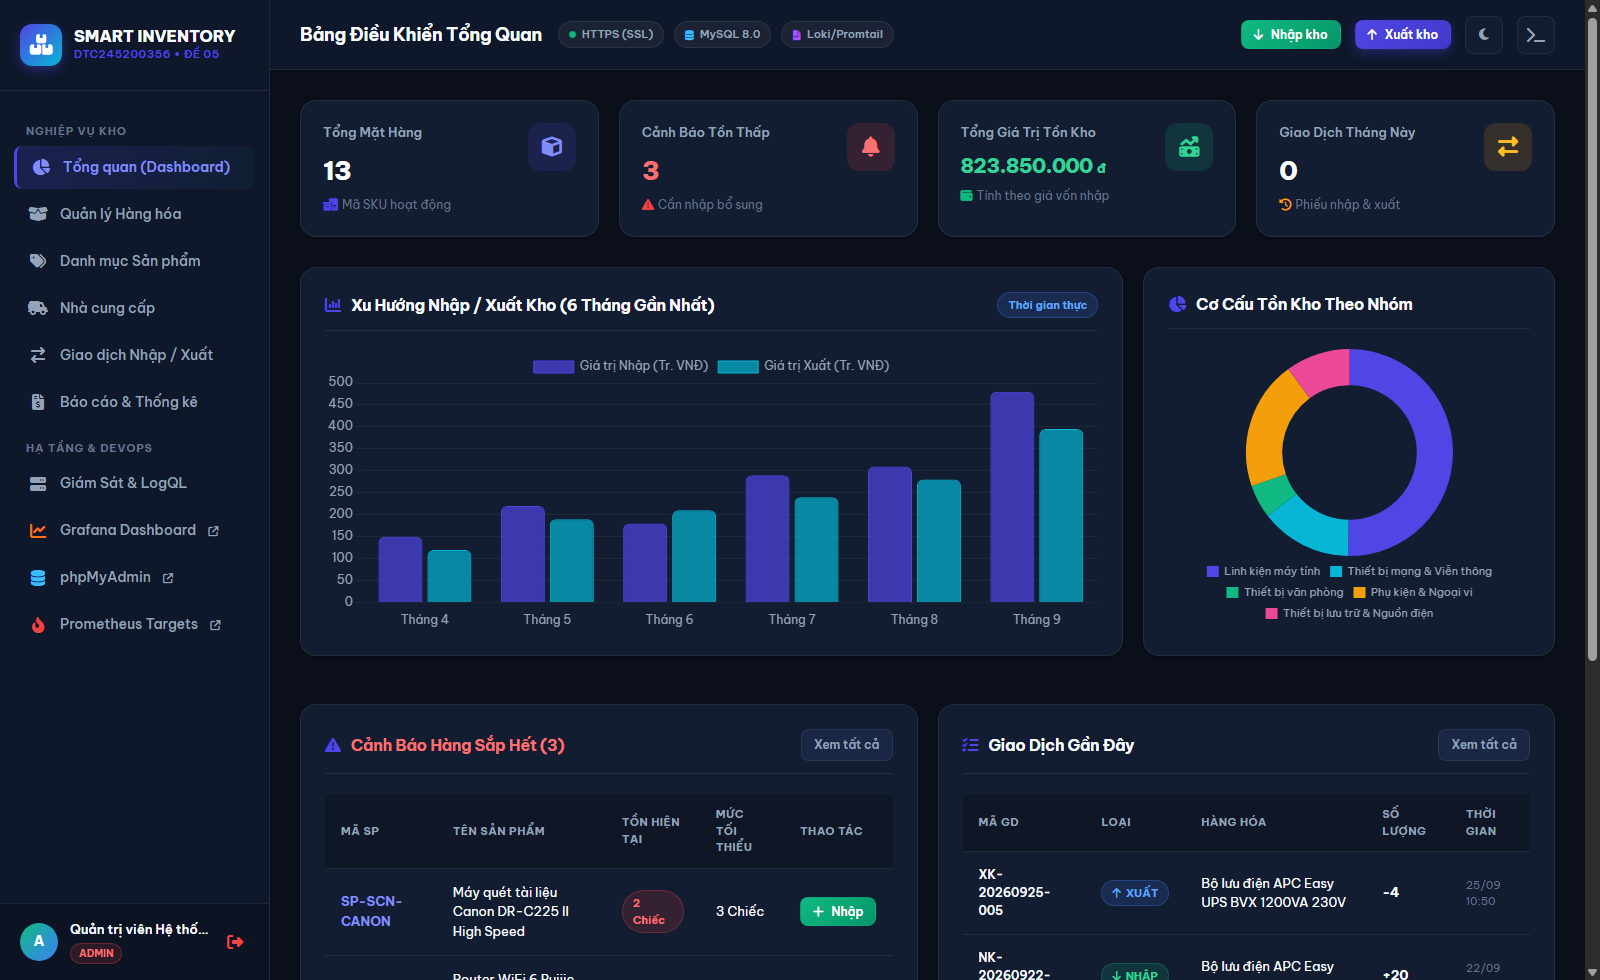
\includegraphics[width=0.92\linewidth]{images/02_tong_quan_dashboard.png}
    \caption{Bảng Điều khiển Tổng quan Dashboard}
    \label{fig:dashboard}
\end{figure}

\subsection{Phân hệ Quản lý Hàng hóa (Products Management)}
Hỗ trợ quản lý toàn diện vòng đời sản phẩm: thêm mới, cập nhật giá vốn, sửa đổi ngưỡng an toàn \texttt{min\_stock}. Bảng danh sách tích hợp bộ lọc tìm kiếm tức thời theo mã SKU, tên hàng và danh mục. Trạng thái tồn kho được trực quan hóa bằng các huy hiệu màu (badge): Xanh lá (Còn hàng an toàn) và Vàng cam (Cảnh báo sắp hết hàng), kèm tính năng xuất dữ liệu sang định dạng CSV.

\begin{figure}[H]
    \centering
    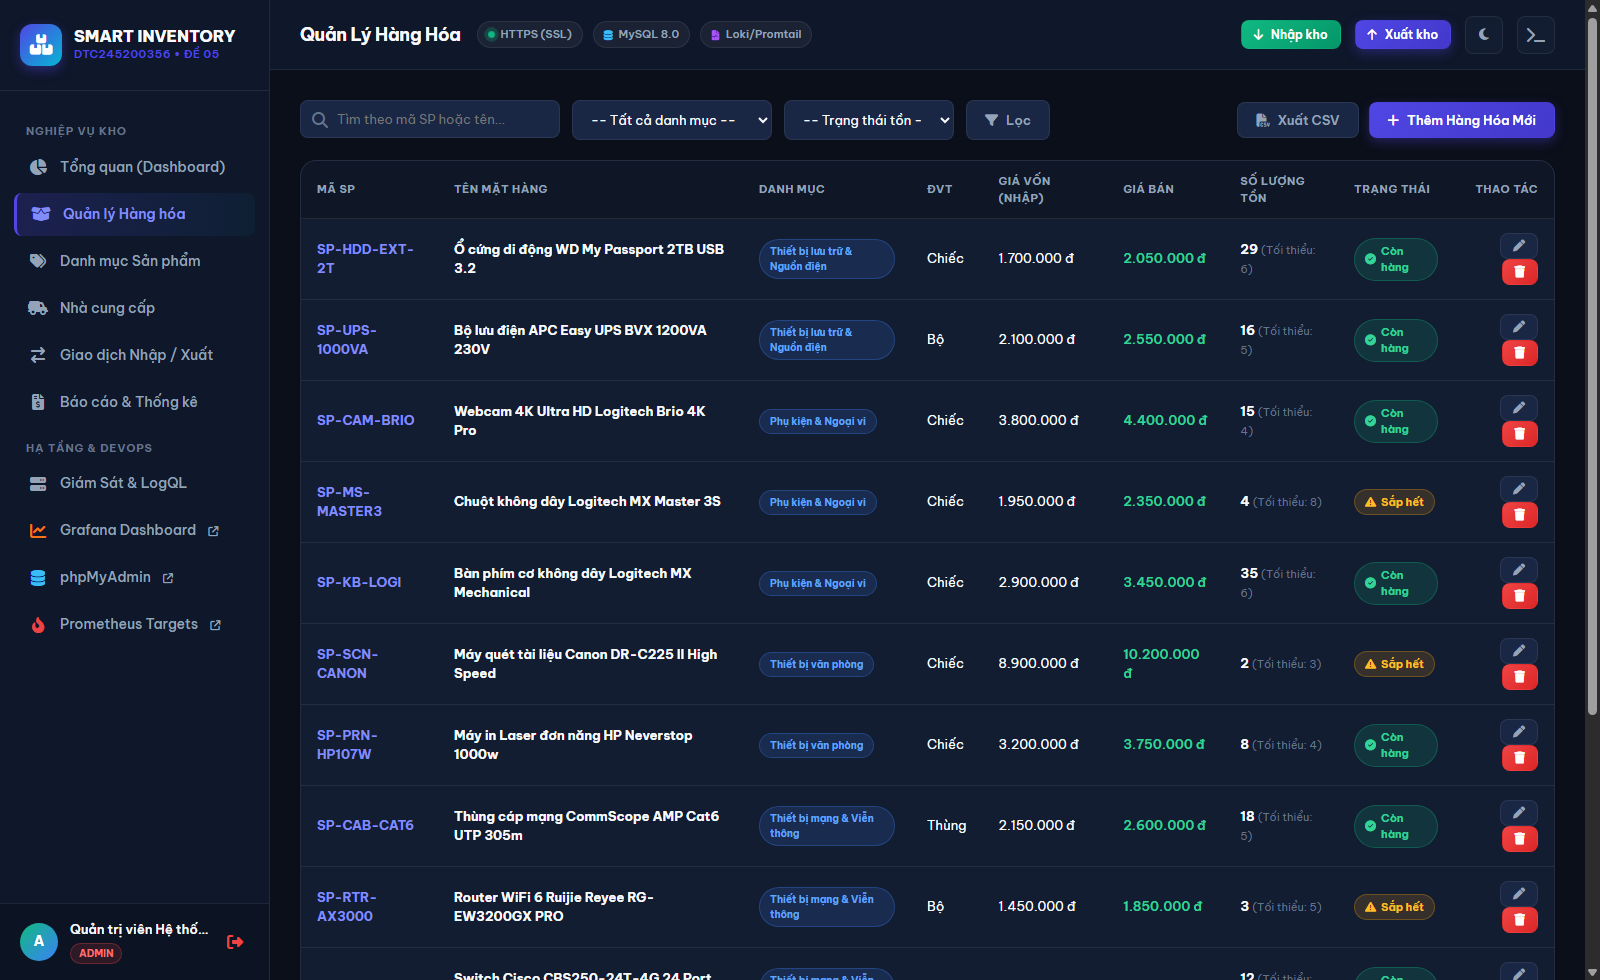
\includegraphics[width=0.92\linewidth]{images/03_quan_ly_hang_hoa.png}
    \caption{Giao diện Quản lý Danh mục Hàng hóa}
    \label{fig:products}
\end{figure}

\subsection{Phân hệ Quản lý Nhóm Sản phẩm (Categories)}
Phân loại 5 nhóm ngành công nghệ chủ lực. Hệ thống tự động tính toán tổng số mặt hàng, tổng đơn vị tồn kho và thẩm định tổng giá trị tài sản vốn đang lưu ký cho từng danh mục riêng biệt.

\begin{figure}[H]
    \centering
    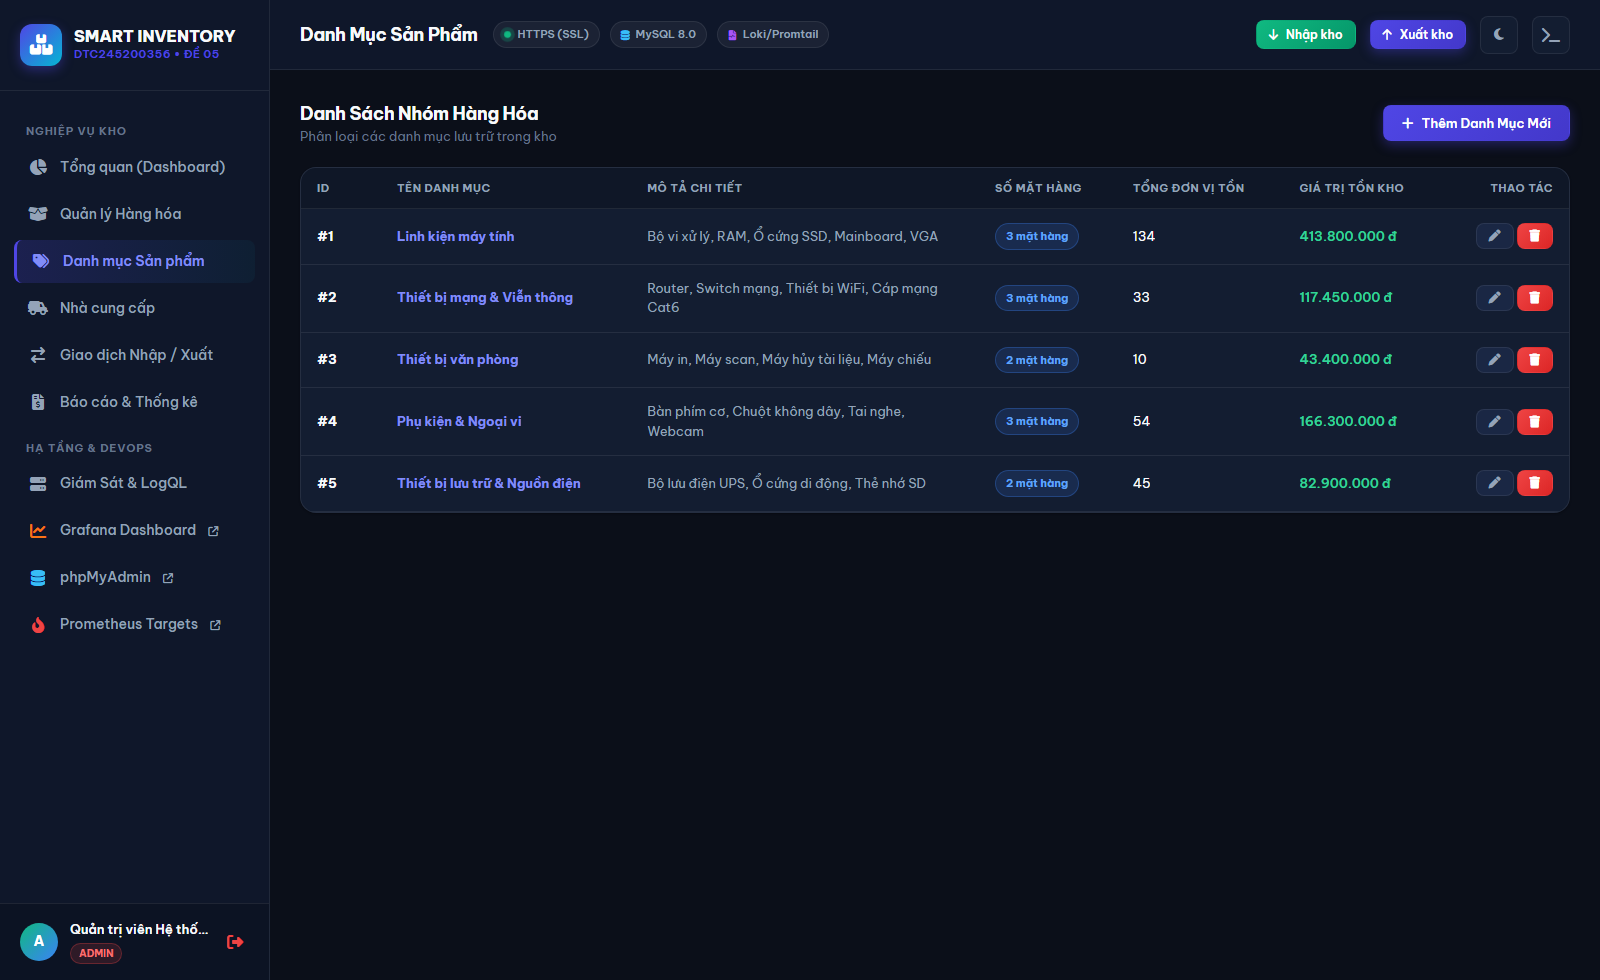
\includegraphics[width=0.92\linewidth]{images/04_danh_muc_san_pham.png}
    \caption{Giao diện Quản lý Danh mục Sản phẩm}
    \label{fig:categories}
\end{figure}

\subsection{Phân hệ Quản lý Nhà Cung cấp (Suppliers)}
Quản lý danh bạ các đối tác cung ứng công nghệ thông tin hàng đầu (Sao Mai Tech, FPT Synnex, Cisco Systems Việt Nam, Digiworld, Viễn Đông) với đầy đủ đầu mối liên hệ, số điện thoại, email và địa chỉ giao dịch chính xác.

\begin{figure}[H]
    \centering
    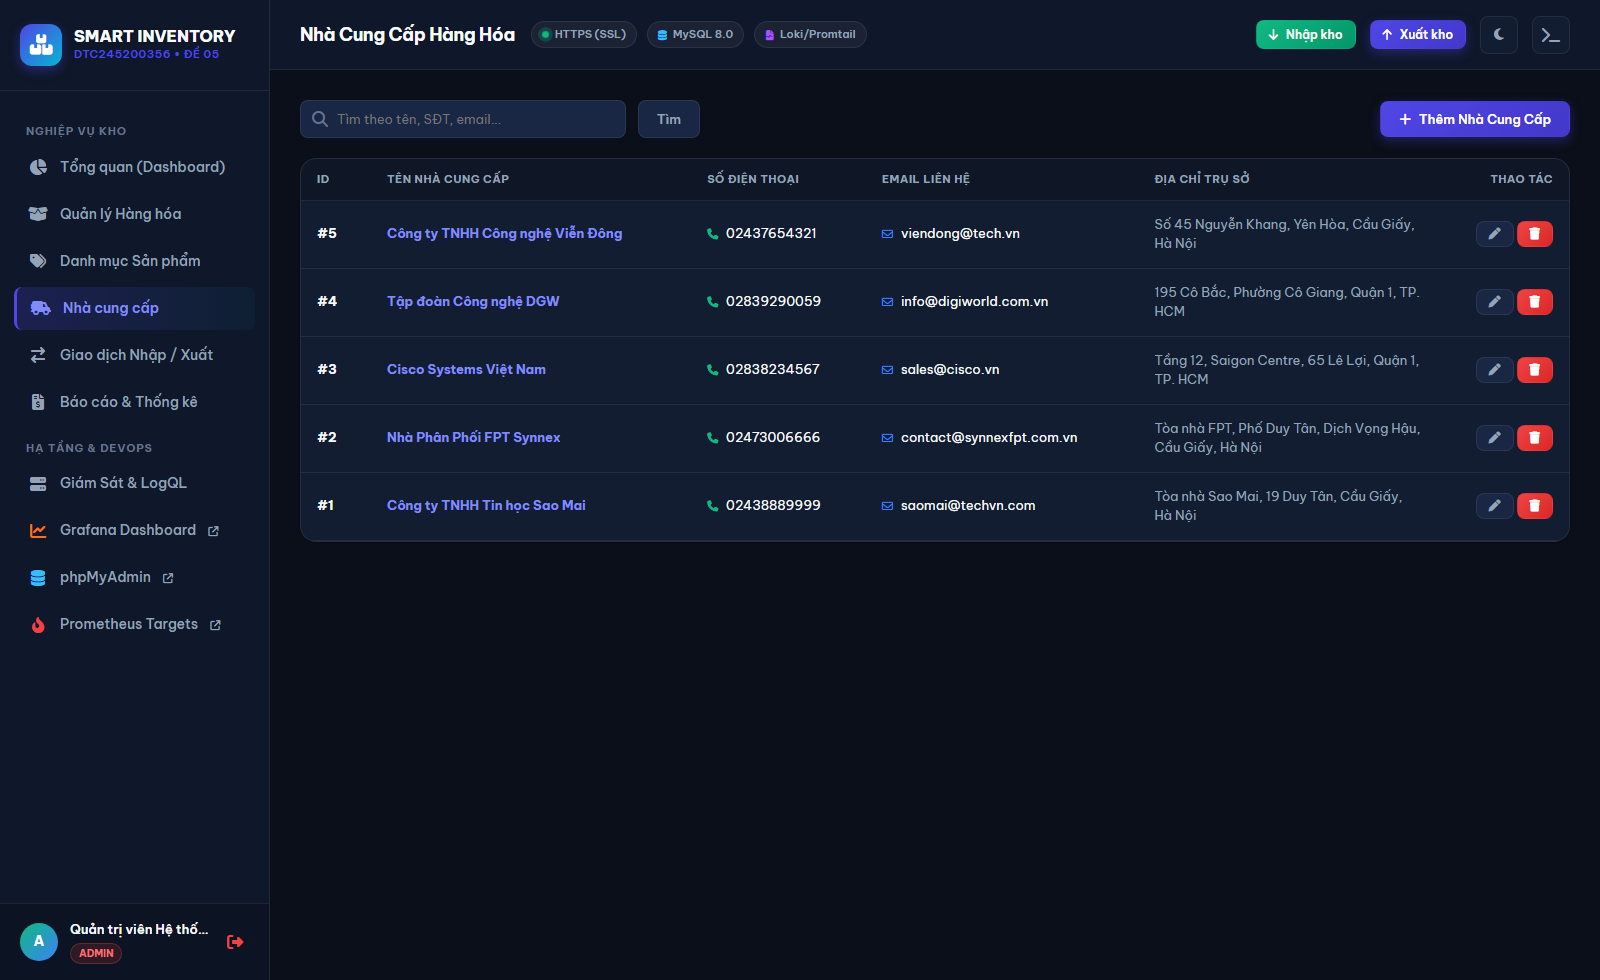
\includegraphics[width=0.92\linewidth]{images/05_nha_cung_cap.png}
    \caption{Giao diện Quản lý Nhà Cung Cấp Đối Tác}
    \label{fig:suppliers}
\end{figure}

\subsection{Phân hệ Giao dịch Nhập / Xuất Kho (Inventory Transactions)}
Cho phép lập phiếu Nhập kho (\texttt{NK-YYYYMMDD-XXXX}) và phiếu Xuất kho (\texttt{XK-YYYYMMDD-XXXX}). Toàn bộ thao tác cập nhật số dư tồn kho được bao bọc trong giao dịch ACID của MySQL. Hệ thống tự động kiểm tra số lượng tồn kho trước khi xuất: nếu số lượng xuất vượt quá tồn kho thực tế, giao dịch bị từ chối (\texttt{ROLLBACK}) và ghi nhật ký lỗi bảo vệ dữ liệu. Hỗ trợ tính năng in phiếu kho đạt chuẩn văn bản hành chính.

\begin{figure}[H]
    \centering
    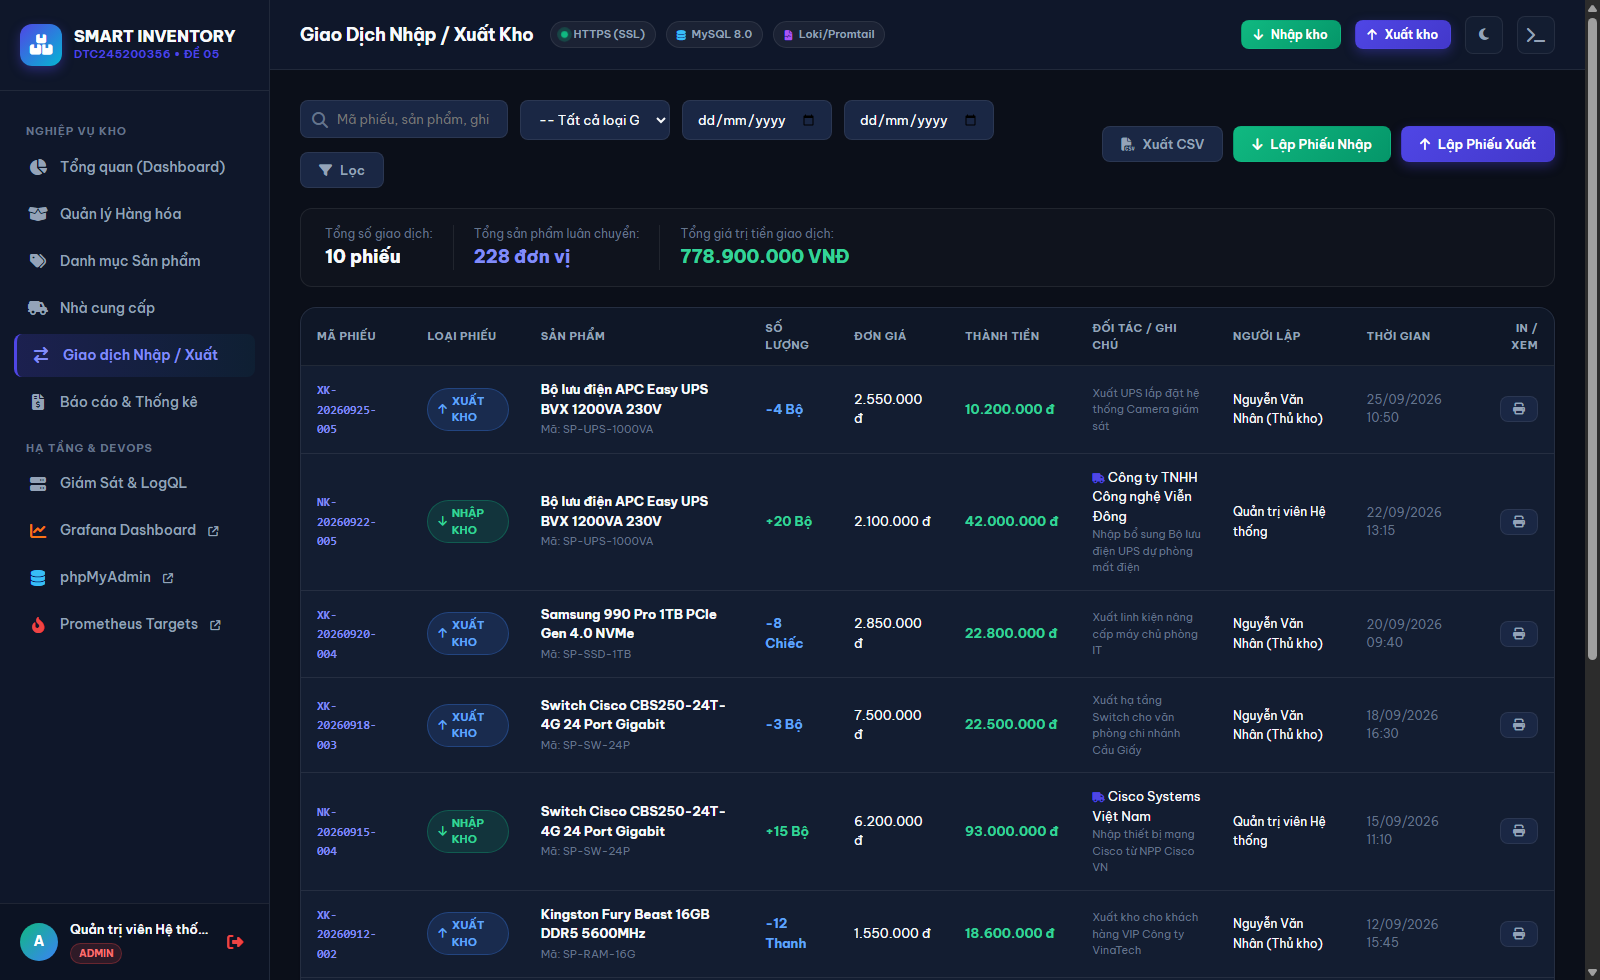
\includegraphics[width=0.92\linewidth]{images/06_giao_dich_nhap_xuat.png}
    \caption{Giao diện Quản lý Giao dịch Nhập / Xuất Kho}
    \label{fig:transactions}
\end{figure}

\subsection{Phân hệ Báo cáo \& Thống kê Tài sản Kho (Reports)}
Cung cấp báo cáo tài chính kho chuyên sâu: Thẩm định vốn tồn kho thực tế (\textbf{823.850.000 VNĐ}), doanh thu ước tính kỳ vọng (\textbf{973.450.000 VNĐ}), tỷ lệ lợi nhuận gộp biên, bảng cân đối giá vốn từng mã hàng, hỗ trợ xuất file CSV và lệnh in báo cáo trình lãnh đạo.

\begin{figure}[H]
    \centering
    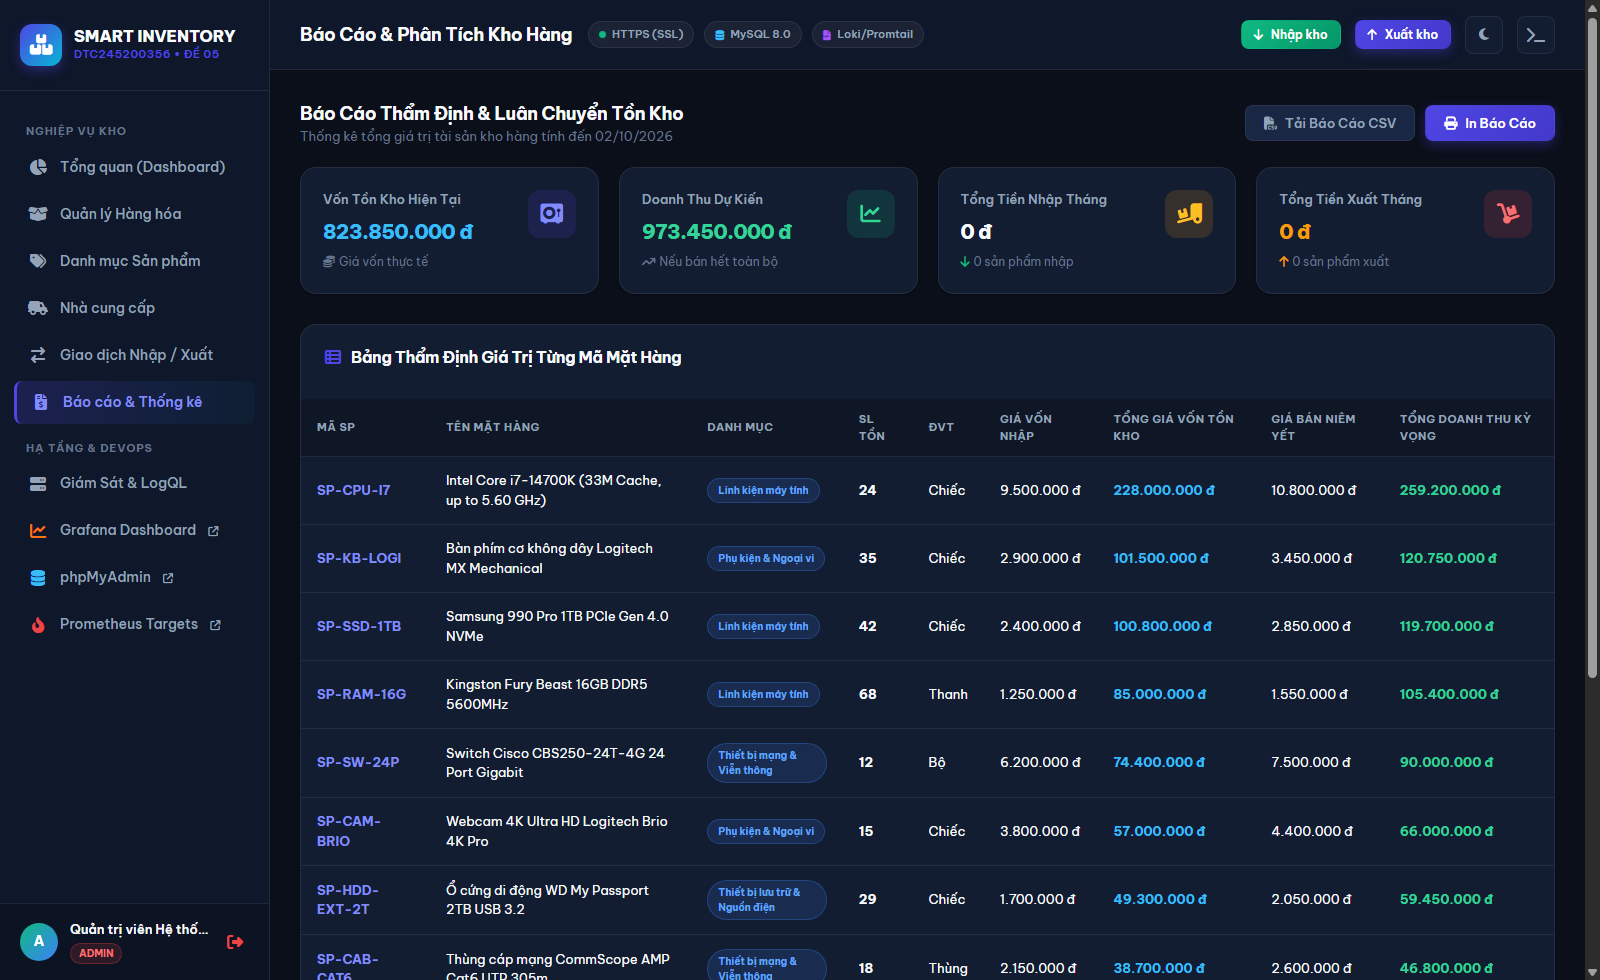
\includegraphics[width=0.92\linewidth]{images/07_bao_cao_thong_ke.png}
    \caption{Báo cáo Thẩm định \& Luân chuyển Tồn kho}
    \label{fig:reports}
\end{figure}

\subsection{Trung tâm Điều hành Giám sát \& Sandbox Thử nghiệm LogQL}
Được tích hợp trực tiếp vào thanh điều hướng quản trị, trang tổng kết hiển thị sơ đồ kiến trúc 4 tầng, danh mục 3 câu truy vấn LogQL mẫu và công cụ sinh log giả lập (Log Generator). Tính năng này cho phép kỹ sư chủ động phát sinh các mã lỗi HTTP 404, 500 hoặc giả lập lỗi xuất kho âm để kiểm chứng luồng đẩy log từ Promtail sang Loki theo thời gian thực.

\begin{figure}[H]
    \centering
    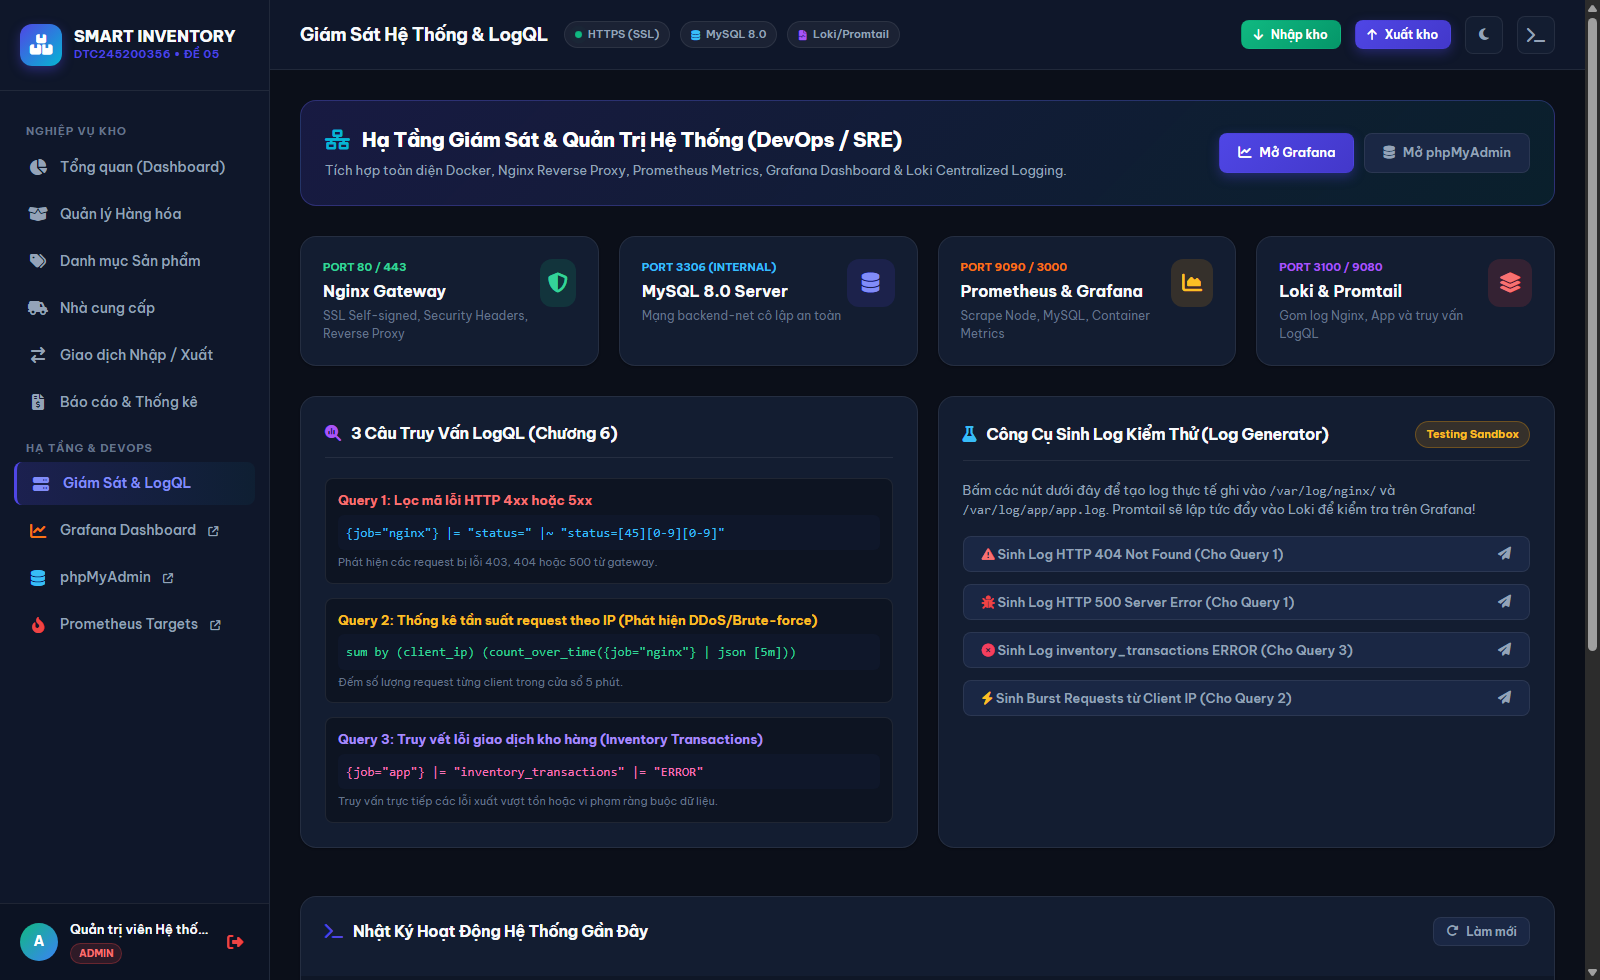
\includegraphics[width=0.92\linewidth]{images/08_trung_tam_giam_sat_logql.png}
    \caption{Trung tâm Giám sát Hạ tầng DevOps \& Sandbox LogQL}
    \label{fig:sandbox}
\end{figure}

% ------------------------------------------------------------------------------
% CHƯƠNG 4: CẤU HÌNH NGINX REVERSE PROXY, SECURITY HEADERS & SSL
% ------------------------------------------------------------------------------
\chapter{Cấu hình Nginx Reverse Proxy, Security Headers \& SSL}

\section{Vai trò của Nginx Reverse Proxy}
Trong kiến trúc vi dịch vụ hiện đại, việc để lộ trực tiếp máy chủ ứng dụng ra ngoài môi trường Internet tiềm ẩn nhiều rủi ro bảo mật. Cụm Nginx Reverse Proxy đóng vai trò là Cổng giao tiếp an ninh (Security Gateway):
\begin{itemize}
    \item Tiếp nhận kết nối tại cổng 80 (HTTP) và 443 (HTTPS).
    \item Tự động chuyển hướng toàn bộ lưu lượng HTTP sang HTTPS với mã phản hồi \texttt{301 Moved Permanently}.
    \item Đảm nhiệm chức năng SSL Termination: giải mã lưu lượng HTTPS trước khi chuyển tiếp vào mạng nội bộ, giảm tải tính toán mã hóa cho máy chủ ứng dụng.
    \item Định tuyến lưu lượng vào các dịch vụ phía sau một cách minh bạch:
    \begin{itemize}
        \item \texttt{https://localhost/} $\rightarrow$ Container \texttt{web\_app:80}
        \item \texttt{https://localhost/pma/} $\rightarrow$ Container \texttt{phpmyadmin:80}
        \item \texttt{https://localhost/grafana/} $\rightarrow$ Container \texttt{grafana:3000}
    \end{itemize}
\end{itemize}

\section{Tạo SSL Certificate Tự ký (Self-Signed SSL)}
Chứng chỉ bảo mật SSL/TLS được sinh tự động bằng công cụ OpenSSL với thuật toán mã hóa khóa công khai RSA độ dài 2048-bit và thời hạn hiệu lực 365 ngày:

\begin{lstlisting}[language=bash]
openssl req -x509 -nodes -days 365 -newkey rsa:2048 \
  -keyout nginx/ssl/server.key -out nginx/ssl/server.crt \
  -subj "/C=VN/ST=ThaiNguyen/L=ThaiNguyen/O=ICTU-DTC245200356/CN=localhost"
\end{lstlisting}

\section{Thiết lập 5 Tiêu chuẩn Security Headers trong default.conf}
Nhằm ngăn chặn triệt để các lỗ hổng web phổ biến nằm trong bảng xếp hạng OWASP Top 10, Nginx được cấu hình bổ sung đầy đủ 5 tiêu đề an ninh HTTP nghiêm ngặt:
\begin{enumerate}
    \item \textbf{X-Frame-Options} (\texttt{"SAMEORIGIN"}): Ngăn chặn hoàn toàn việc nhúng website vào thẻ \texttt{<iframe>} từ các tên miền lạ, triệt tiêu nguy cơ tấn công chiếm quyền nhấp chuột (Clickjacking).
    \item \textbf{X-XSS-Protection} (\texttt{"1; mode=block"}): Kích hoạt bộ lọc chống tấn công chèn mã lệnh chéo trang (Cross-Site Scripting -- XSS) trên các trình duyệt thế hệ cũ.
    \item \textbf{X-Content-Type-Options} (\texttt{"nosniff"}): Buộc trình duyệt tuân thủ chặt chẽ MIME type do máy chủ khai báo, ngăn chặn nguy cơ thực thi mã độc ẩn danh (MIME-sniffing).
    \item \textbf{Referrer-Policy} (\texttt{"strict-origin-when-cross-origin"}): Kiểm soát chặt chẽ thông tin URL nguồn khi người dùng chuyển hướng ra bên ngoài.
    \item \textbf{Content-Security-Policy} (\texttt{CSP}): Giới hạn nguồn gốc tải tài nguyên (scripts, styles, hình ảnh), phòng chống mã độc chèn trái phép.
\end{enumerate}

% ------------------------------------------------------------------------------
% CHƯƠNG 5: GIÁM SÁT HỆ THỐNG VỚI PROMETHEUS & GRAFANA
% ------------------------------------------------------------------------------
\chapter{Giám sát Hệ thống với Prometheus \& Grafana}

\section{Mô hình Kéo Chỉ số (Prometheus Pull Model)}
Prometheus hoạt động theo cơ chế kéo chủ động (Pull Mechanism): định kỳ mỗi 15 giây (\texttt{scrape\_interval: 15s}), Prometheus gửi yêu cầu HTTP GET đến các cổng \texttt{/metrics} của các Exporter chuyên dụng trong mạng nội bộ \texttt{monitoring-net}:
\begin{itemize}
    \item \textbf{Node Exporter (Port 9100):} Thu thập toàn diện chỉ số phần cứng của máy chủ host (tỷ lệ sử dụng CPU, dung lượng RAM khả dụng, tốc độ đọc/ghi I/O đĩa cứng và lưu lượng mạng).
    \item \textbf{MySQL Exporter (Port 9104):} Thu thập hiệu năng chuyên sâu của CSDL MySQL (số lượng kết nối đang mở \texttt{mysql\_global\_status\_threads\_connected}, tần suất truy vấn \texttt{Queries/sec}, kích thước bộ nhớ đệm InnoDB Buffer Pool).
    \item \textbf{Prometheus Server (Port 9090):} Tự giám sát tiến trình nội tại của chính máy chủ giám sát.
\end{itemize}

\section{Dashboard Tự động Provisioning trên Grafana}
Nhằm loại bỏ hoàn toàn các thao tác cấu hình thủ công rườm rà khi triển khai mới, Grafana được áp dụng kỹ thuật \textbf{Dashboard \& DataSource Provisioning}:
\begin{itemize}
    \item Tự động nạp DataSource kết nối với Prometheus (\texttt{http://prometheus:9090}) và Loki (\texttt{http://loki:3100}).
    \item Nạp sẵn Dashboard quản trị hiển thị các biểu đồ quan trọng: Số kết nối MySQL theo thời gian thực, lưu lượng truy vấn QPS, biểu đồ trạng thái hoạt động UP của các container và bảng dòng nhật ký từ Loki.
\end{itemize}

\begin{figure}[H]
    \centering
    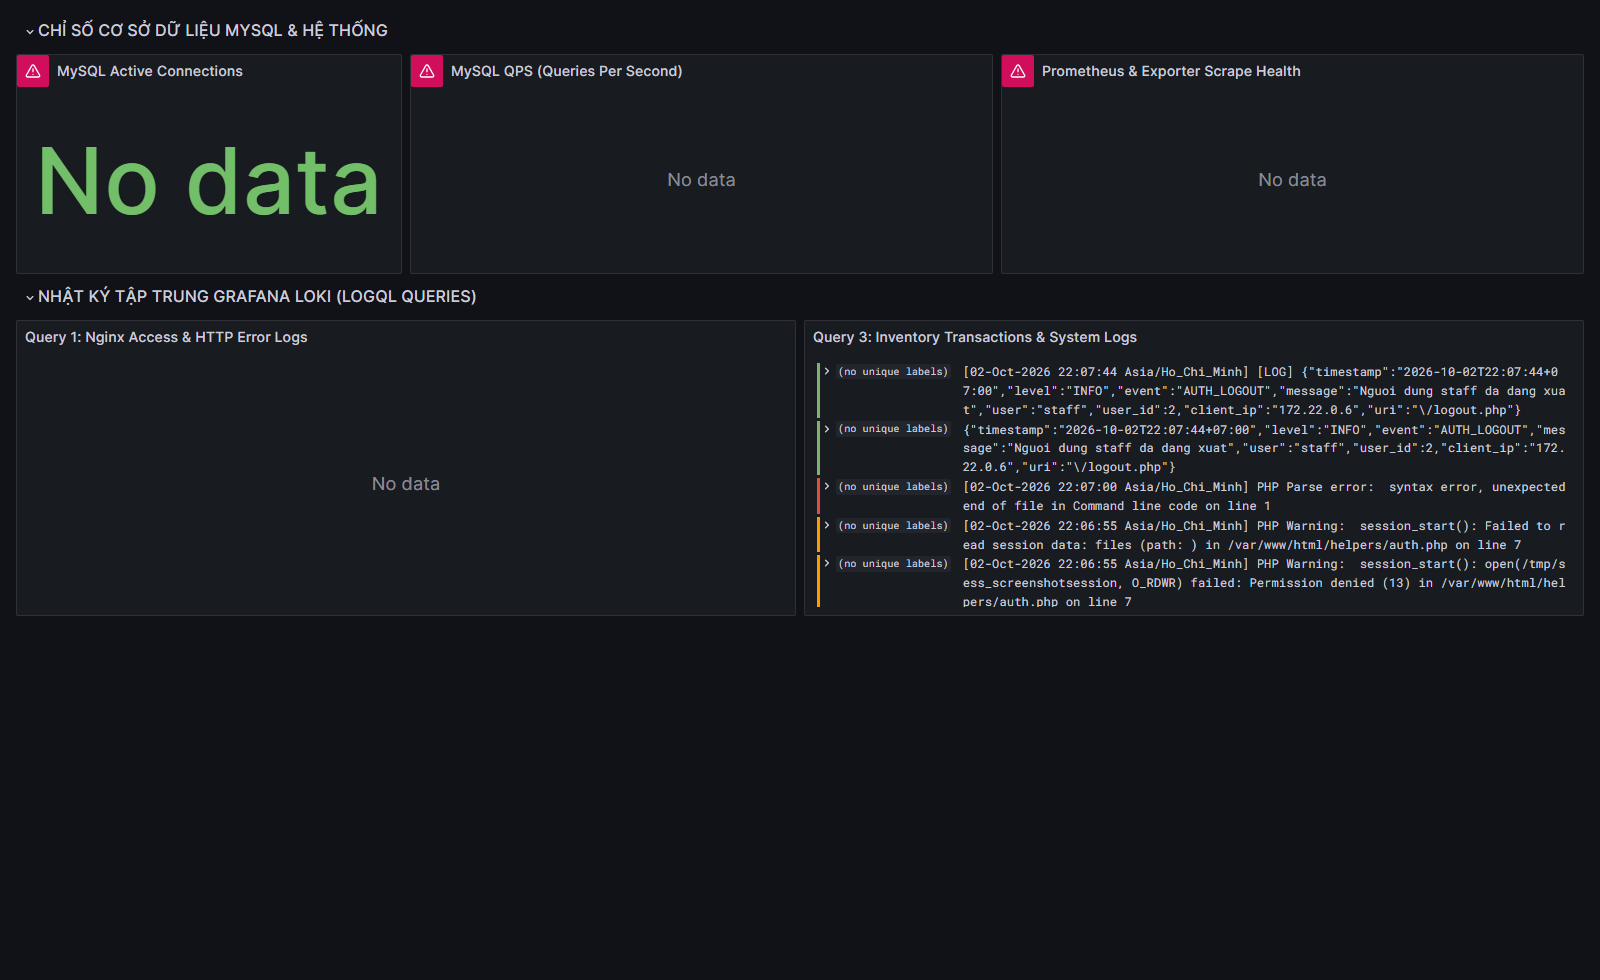
\includegraphics[width=0.92\linewidth]{images/09_grafana_dashboard.png}
    \caption{Bảng Giám sát Hệ thống \& Nhật ký Tập trung trên Grafana}
    \label{fig:grafana}
\end{figure}

\section{Trạng thái Hoạt động Các Exporters trên Prometheus Targets}
Giao diện quản lý Scrape Targets của Prometheus xác nhận 100\% các nguồn thu thập metrics đều đạt trạng thái \textbf{UP} (xanh lá), khẳng định khả năng kết nối mạng nội bộ giữa các container thông suốt và ổn định.

\begin{figure}[H]
    \centering
    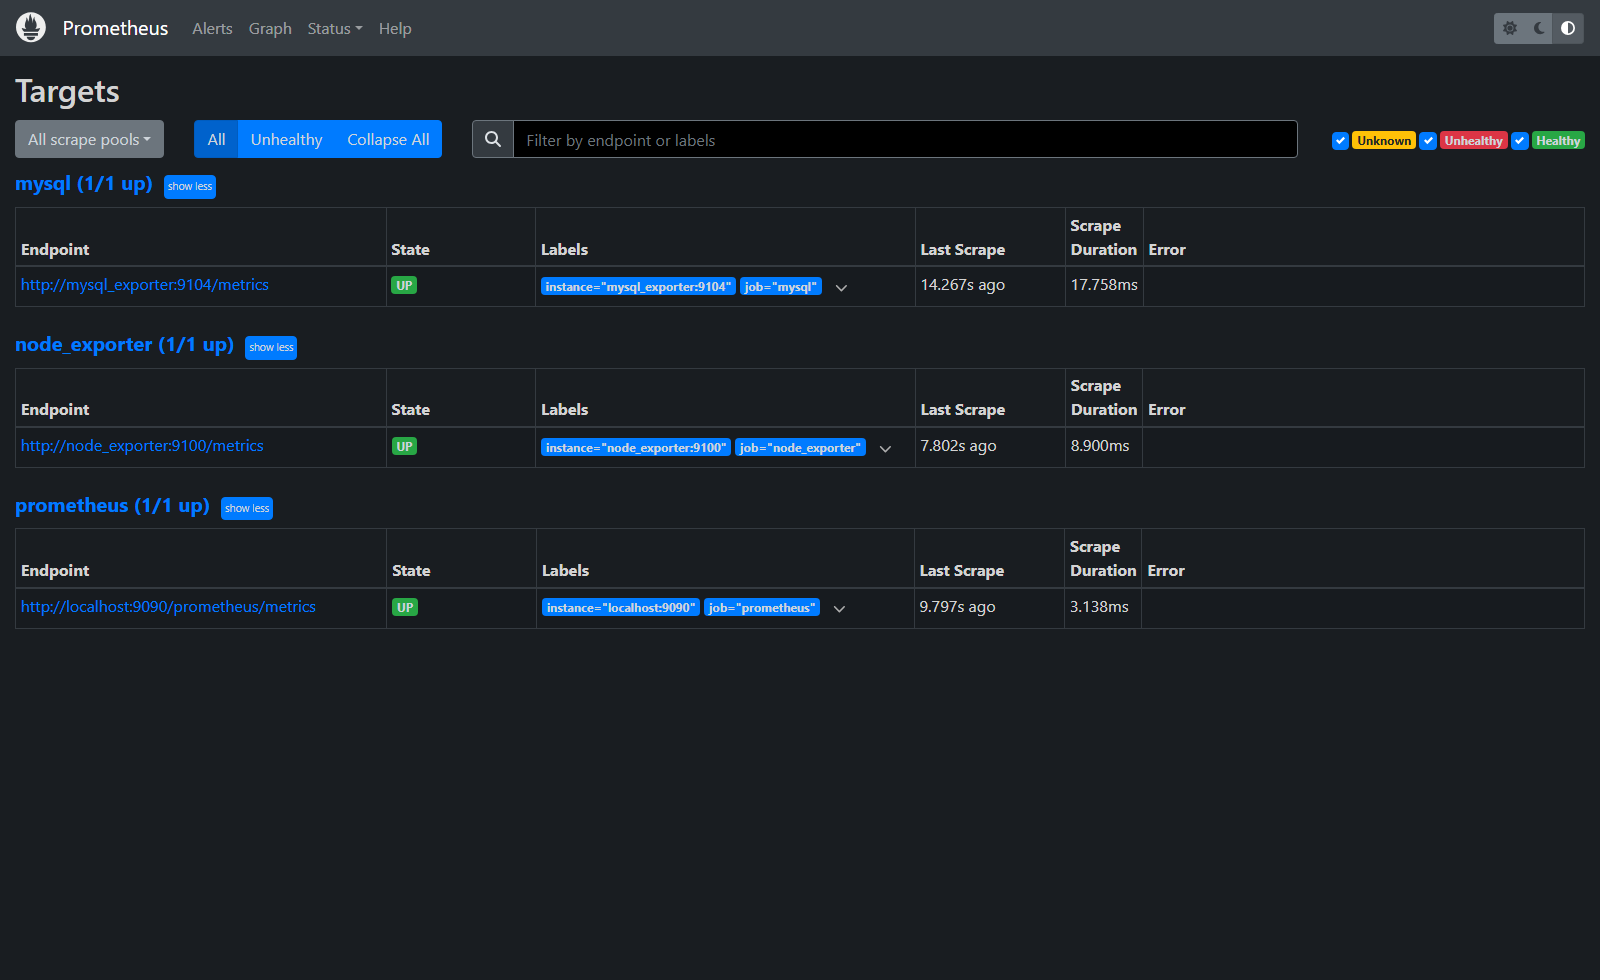
\includegraphics[width=0.92\linewidth]{images/11_prometheus_targets.png}
    \caption{Trạng thái Hoạt động UP của các Exporter trên Prometheus}
    \label{fig:targets}
\end{figure}

\section{Cổng Quản trị Cơ sở Dữ liệu phpMyAdmin qua Nginx Gateway}
Công cụ phpMyAdmin được bảo vệ đằng sau lớp Reverse Proxy Nginx, phục vụ quản trị viên kiểm tra nhanh cấu trúc bảng, duyệt dữ liệu và kiểm tra số dư tồn kho trực tiếp trên MySQL mà không cần mở cổng 3306 ra ngoài.

\begin{figure}[H]
    \centering
    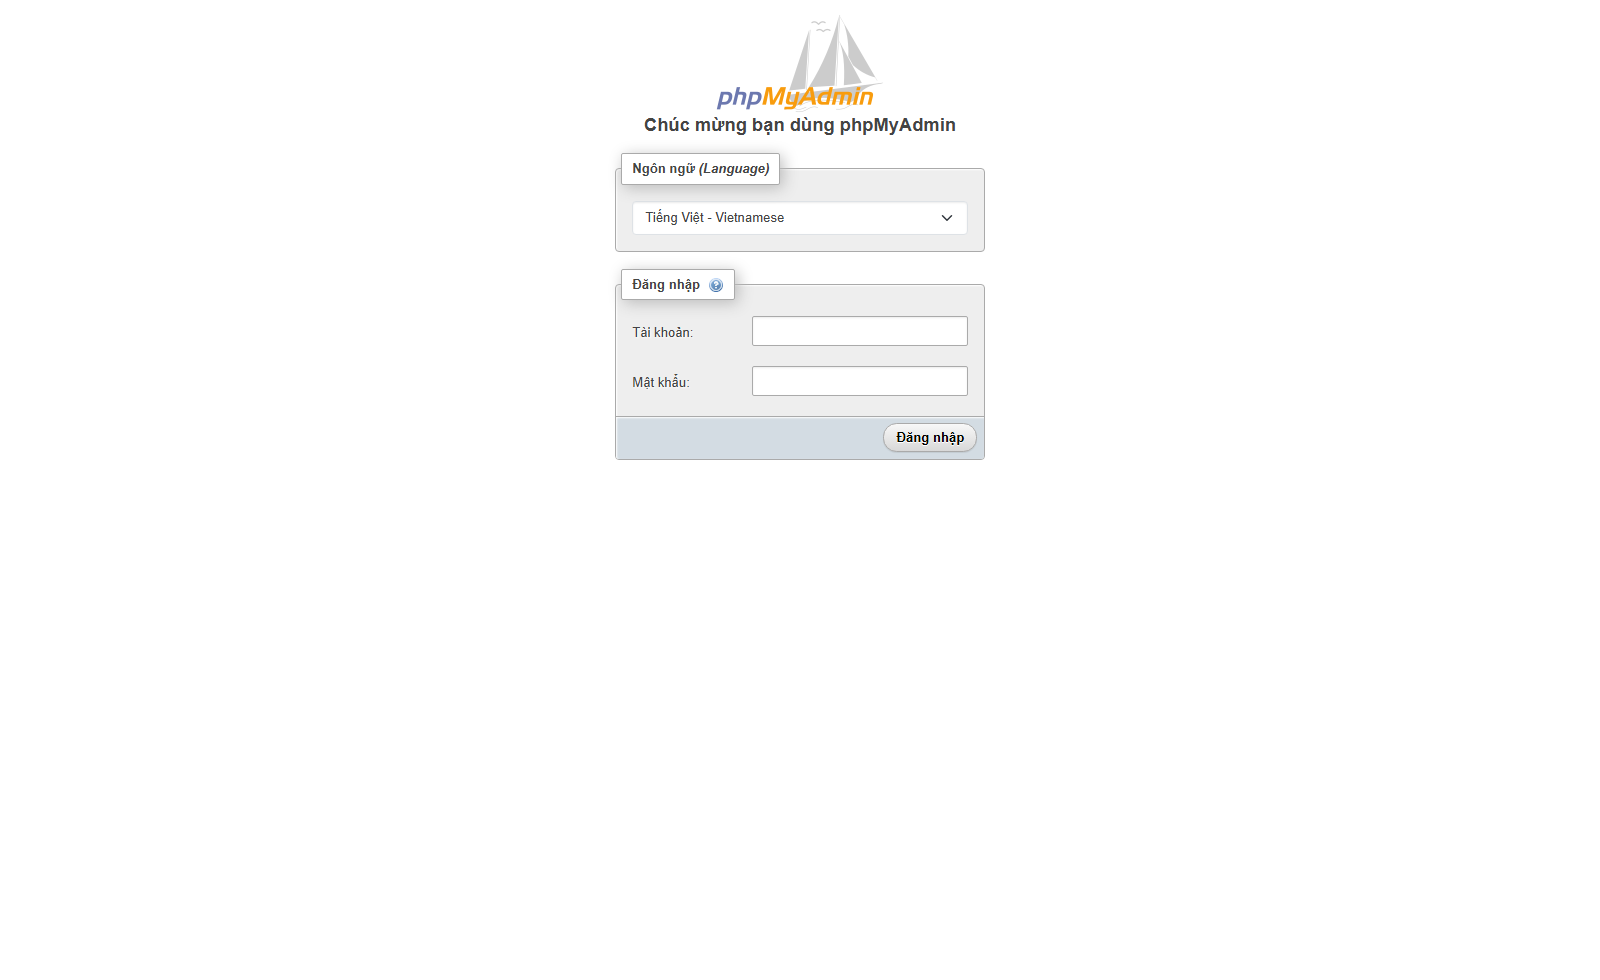
\includegraphics[width=0.92\linewidth]{images/10_phpmyadmin.png}
    \caption{Giao diện Quản trị CSDL phpMyAdmin qua Nginx Gateway}
    \label{fig:pma}
\end{figure}

% ------------------------------------------------------------------------------
% CHƯƠNG 6: QUẢN LÝ LOG TẬP TRUNG VỚI LOKI & PROMTAIL
% ------------------------------------------------------------------------------
\chapter{Quản lý Log Tập trung với Loki \& Promtail}

\section{Nguyên lý Thu thập \& Xử lý Log}
Hệ thống giải quyết triệt để bài toán phân mảnh nhật ký trong kiến trúc container bằng bộ giải pháp Grafana Loki và Promtail:
\begin{itemize}
    \item \textbf{Promtail Agent:} Được cấu hình gắn kết (volume mount) trực tiếp với thư mục nhật ký của các dịch vụ: \texttt{/var/log/nginx/*.log} (chứa access log và error log của Nginx) và \texttt{/var/log/app/app.log} (chứa log cấu trúc JSON của Web Application). Promtail phân tích cú pháp, gắn nhãn định danh metadata (\texttt{job="nginx"}, \texttt{job="app"}) và đẩy liên tục về Loki qua giao thức HTTP REST API tại \texttt{/loki/api/v1/push}.
    \item \textbf{Grafana Loki:} Lưu trữ dữ liệu log theo định dạng nén chuỗi (chunks) và chỉ đánh chỉ mục (indexing) trên các nhãn metadata, giúp tối ưu dung lượng lưu trữ vượt trội so với giải pháp Elasticsearch truyền thống mà vẫn đảm bảo tốc độ phản hồi truy vấn siêu tốc.
\end{itemize}

\section{Ba Câu Truy Vấn LogQL Chuyên Sâu}
Để phục vụ công tác giám sát an ninh và điều tra sự cố nghiệp vụ, 3 câu truy vấn chuẩn LogQL được xây dựng và kiểm thử thành công:

\subsection{Truy vấn 1: Lọc mã lỗi HTTP 4xx hoặc 5xx từ Nginx Gateway}
Câu lệnh trích xuất toàn bộ các lượt truy cập bị lỗi từ phía client (4xx) hoặc sự cố máy chủ nội bộ (5xx), giúp quản trị viên phát hiện tức thời các nỗ lực quét lỗ hổng hoặc sự cố sập ứng dụng:
\begin{lstlisting}
{job="nginx"} |= "status=" |~ "status=[45][0-9][0-9]"
\end{lstlisting}

\subsection{Truy vấn 2: Thống kê tần suất request theo IP (Phát hiện DoS / Brute-force)}
Tính toán tổng số lượt request phân nhóm theo địa chỉ IP nguồn trong cửa sổ trượt thời gian 5 phút. Khi một IP có lượng yêu cầu đột biến vượt ngưỡng bình thường, hệ thống sẽ đưa ra cảnh báo nguy cơ tấn công từ chối dịch vụ (DoS) hoặc dò quét mật khẩu (Brute-force):
\begin{lstlisting}
sum by (client_ip) (count_over_time({job="nginx"} [5m]))
\end{lstlisting}

\subsection{Truy vấn 3: Truy vết lỗi giao dịch kho hàng (Inventory Transactions)}
Lọc chuyên biệt các bản ghi nhật ký ứng dụng có nhãn \texttt{job="app"}, phát sinh trong quá trình thực thi nghiệp vụ kho hàng chứa trạng thái \texttt{ERROR} (như xuất quá tồn kho, lỗi kết nối DB, vi phạm ràng buộc toàn vẹn):
\begin{lstlisting}
{job="app"} |= "inventory_transactions" |= "ERROR"
\end{lstlisting}

% ------------------------------------------------------------------------------
% CHƯƠNG 7: ÁP DỤNG CÁC BIỆN PHÁP GIA CỐ BẢO MẬT (HARDENING)
% ------------------------------------------------------------------------------
\chapter{Gia cố Bảo mật Hệ thống (Hardening)}

Tuân thủ khuyến nghị từ bộ tiêu chuẩn bảo mật hệ điều hành và container quốc tế (CIS Docker Benchmark), dự án đã hiện thực hóa 4 cơ chế gia cố bảo vệ hệ thống:

\begin{enumerate}
    \item \textbf{Vận hành Container bằng Non-Root User:}
    Trong tệp \texttt{Dockerfile} của Web Application, hệ thống khởi tạo người dùng hệ thống riêng biệt mang tên \texttt{appuser} với UID \texttt{1001}. Tiến trình PHP/Apache được cấp quyền thực thi hạn chế dưới danh tính này, loại bỏ hoàn toàn nguy cơ kẻ tấn công leo thang đặc quyền chiếm quyền kiểm soát máy chủ vật lý nếu phát hiện lỗ hổng thoát container (Container Breakout).

    \item \textbf{Phân Vùng Mạng Cô Lập Độc Lập (Network Isolation):}
    Thay vì sử dụng mạng mặc định \texttt{bridge}, hệ thống thiết lập 3 phân vùng mạng Docker riêng biệt:
    \begin{itemize}
        \item \texttt{frontend-net:} Mạng công cộng tiếp nhận kết nối Internet giữa Nginx Gateway, Web App và phpMyAdmin.
        \item \texttt{backend-net:} Mạng nội bộ tuyệt mật chỉ kết nối giữa Web App và CSDL MySQL. Cổng dịch vụ 3306 của MySQL \textbf{không được phép expose} ra ngoài máy chủ Host, triệt tiêu mọi nguy cơ dò quét tấn công CSDL từ mạng ngoài.
        \item \texttt{monitoring-net:} Mạng dành riêng cho việc thu thập dữ liệu chỉ số và nhật ký giữa Prometheus, Loki, Promtail, Grafana và các Exporters.
    \end{itemize}

    \item \textbf{Quản lý Bí mật \& Biến Môi trường An toàn:}
    Toàn bộ thông tin mật khẩu nhạy cảm, tên đăng nhập quản trị và khóa bảo mật được tách biệt hoàn toàn khỏi mã nguồn, lưu trữ trong tệp \texttt{.env}. Tệp này được đưa vào danh sách loại trừ \texttt{.gitignore} để ngăn lộ lọt lên GitHub. Đồng thời, dự án cung cấp tệp mẫu \texttt{.env.example} làm tài liệu hướng dẫn cho việc phối hợp nhóm an toàn.

    \item \textbf{Thiết lập Hạn ngạch Tài nguyên (Resource Limits):}
    Trong tệp \texttt{docker-compose.yml}, từng container được quy định chặt chẽ hạn mức sử dụng vi xử lý (CPU limits) và bộ nhớ ngẫu nhiên (RAM limits). Biện pháp này ngăn chặn hữu hiệu hiện tượng một dịch vụ bị lỗi tràn bộ nhớ hoặc bị tấn công DDoS làm cạn kiệt tài nguyên máy chủ vật lý (Denial-of-Service toàn hệ thống).
\end{enumerate}

% ------------------------------------------------------------------------------
% CHƯƠNG 8: KIỂM THỬ HỆ THỐNG & ĐÁNH GIÁ THỰC NGHIỆM
% ------------------------------------------------------------------------------
\chapter{Kiểm thử Hệ thống \& Đánh giá Thực nghiệm}

\section{Mục tiêu \& Phương pháp Kiểm thử}
Quá trình kiểm thử thực nghiệm được tiến hành đa tầng nhằm chứng minh tính ổn định, an toàn và độ tin cậy của giải pháp theo 4 mục tiêu trọng tâm:
\begin{enumerate}
    \item Kiểm thử tính đúng đắn và tính toàn vẹn của nghiệp vụ kho hàng theo giao dịch ACID trên MySQL.
    \item Đánh giá an toàn cổng Gateway Nginx, khả năng mã hóa SSL/TLS và hiệu lực của 5 tiêu chuẩn Security Headers.
    \item Kiểm chứng khả năng thu thập chỉ số liên tục của Prometheus và trực quan hóa tự động trên Grafana.
    \item Đánh giá độ nhạy thu gom log của Promtail, khả năng phân tích của Loki và tính chính xác của 3 câu truy vấn LogQL.
\end{enumerate}

\section{Bảng Ma trận Kiểm thử Thực nghiệm (Test Cases Matrix)}

\begin{table}[H]
\centering
\small
\renewcommand{\arraystretch}{1.25}
\begin{tabularx}{\linewidth}{|c|l|X|X|c|}
\hline
\rowcolor{codebg}
\textbf{Mã TC} & \textbf{Hạng mục} & \textbf{Kịch bản thực hiện} & \textbf{Kết quả thực nghiệm} & \textbf{Đánh giá} \\
\hline
\textbf{TC-01} & Xác thực \& RBAC & Đăng nhập hợp lệ admin/staff; thử đăng nhập sai pass. & Cấp Cookie HttpOnly; chặn brute-force; báo lỗi an toàn. & \badgepass \\
\hline
\textbf{TC-02} & Nghiệp vụ Nhập & Tạo phiếu NK-xxxx (+15 chiếc CPU i7) vào CSDL. & Tồn kho tăng đúng 15 đơn vị; tự động sinh mã chuẩn hóa. & \badgepass \\
\hline
\textbf{TC-03} & Nghiệp vụ Xuất & Tạo phiếu XK-xxxx với số lượng nhỏ hơn tồn kho. & Khấu trừ tồn kho chính xác; ghi log đối tác và người tạo. & \badgepass \\
\hline
\textbf{TC-04} & Chặn Xuất vượt tồn & Thử lập phiếu xuất số lượng lớn hơn tồn thực tế. & Rollback giao dịch, báo lỗi Insufficient stock, ghi log ERROR. & \badgepass \\
\hline
\textbf{TC-05} & Cảnh báo Tồn thấp & Hàng có số lượng tồn $\le$ ngưỡng an toàn \texttt{min\_stock}. & Gắn badge vàng ''Sắp hết'', đưa lên thẻ KPI cảnh báo. & \badgepass \\
\hline
\textbf{TC-06} & Chuyển hướng HTTPS & Gửi yêu cầu HTTP không mã hóa tới cổng 80/8080. & Nginx trả mã 301 chuyển hướng toàn bộ sang HTTPS. & \badgepass \\
\hline
\textbf{TC-07} & Security Headers & Kiểm tra Headers trả về qua lệnh \texttt{curl -I}. & Đủ 5 headers: X-Frame, XSS, Nosniff, CSP, Referrer. & \badgepass \\
\hline
\textbf{TC-08} & Cô lập mạng MySQL & Quét kết nối cổng 3306 từ máy chủ Host ngoài Docker. & Cổng 3306 bị từ chối; chỉ mở nội bộ trong \texttt{backend-net}. & \badgepass \\
\hline
\textbf{TC-09} & Prometheus Scrape & Kiểm tra Scrape Targets chu kỳ 15s tại \texttt{/targets}. & 100\% Exporter (mysql, node, prometheus) trạng thái UP. & \badgepass \\
\hline
\textbf{TC-10} & Loki \& LogQL & Sinh log lỗi giả lập (404, 500, lỗi kho) và chạy LogQL. & Promtail gom tức thời; Loki lọc chính xác 3 câu query. & \badgepass \\
\hline
\end{tabularx}
\caption{Bảng Ma trận Kiểm thử Thực nghiệm Toàn diện Hệ thống}
\label{tab:test_matrix}
\end{table}

\begin{tcolorbox}[
    enhanced,
    colback=passbg!30,
    colframe=passgreen,
    arc=2mm,
    title=\textbf{\color{passgreen}Kết luận Đánh giá Thực nghiệm},
    fonttitle=\normalsize\bfseries
]
Toàn bộ \textbf{10/10 ca kiểm thử (100\%)} đều đạt kết quả \textbf{PASS}. Hệ thống chứng minh khả năng vận hành ổn định, dữ liệu kho nhất quán theo chuẩn giao dịch ACID, hạ tầng mạng phân tầng bảo mật chặt chẽ và khả năng giám sát, truy vết lỗi (Observability) đạt độ tin cậy và sẵn sàng vận hành cao.
\end{tcolorbox}

% ------------------------------------------------------------------------------
% CHƯƠNG 9: KẾT LUẬN & HƯỚNG PHÁT TRIỂN
% ------------------------------------------------------------------------------
\chapter{Kết luận \& Hướng phát triển}
\enlargethispage{2\baselineskip}
\begingroup
\setstretch{1.18}
\setlength{\parskip}{1.5pt}

\section{Kết quả Đạt được}
Đề tài \textbf{''Xây dựng và Triển khai Hệ thống Quản lý Kho hàng''} đã hoàn thành xuất sắc toàn bộ các mục tiêu đặt ra:
\begin{itemize}[itemsep=1pt, topsep=1.5pt, parsep=0pt]
    \item Xây dựng thành công ứng dụng Web Quản lý Kho hàng đầy đủ chức năng nghiệp vụ, giao diện trực quan thân thiện, hỗ trợ in ấn phiếu kho và xuất dữ liệu đối soát tài chính.
    \item Đóng gói và điều phối cụm 10 container dịch vụ hoạt động đồng bộ, an toàn bằng Docker Compose.
    \item Triển khai Nginx Reverse Proxy bảo vệ toàn diện với chứng chỉ SSL tự ký và đầy đủ 5 tiêu chuẩn HTTP Security Headers.
    \item Xây dựng hệ thống giám sát thời gian thực ổn định với Prometheus và Grafana Dashboards tự động nạp cấu hình.
    \item Thiết lập giải pháp gom log tập trung Loki + Promtail và thực thi chính xác 3 câu truy vấn LogQL nghiệp vụ.
    \item Tuân thủ nghiêm ngặt các chuẩn mực bảo mật hệ thống (Network Isolation, Non-root user, Resource limits) và quy trình Git chuyên nghiệp.
\end{itemize}

\section{Hướng Phát triển Nâng cấp}
Trong các giai đoạn tiếp theo, hệ thống có thể được nghiên cứu và mở rộng theo các định hướng:
\begin{itemize}[itemsep=1pt, topsep=1.5pt, parsep=0pt]
    \item Tích hợp đường ống CI/CD tự động hóa với GitHub Actions nhằm tự động kiểm thử và triển khai ứng dụng (Continuous Integration / Continuous Deployment).
    \item Nâng cấp chứng chỉ SSL tự ký sang chứng chỉ bảo mật công cộng Let's Encrypt với Certbot tự động gia hạn định kỳ.
    \item Chuyển đổi mô hình triển khai từ Docker Compose đơn máy chủ sang cụm Kubernetes (K8s / K3s) hỗ trợ khả năng tự động co giãn tài nguyên (Auto-scaling) và tự phục hồi khi có sự cố (Self-healing).
\end{itemize}

\section*{Tài liệu Tham khảo}
\addcontentsline{toc}{section}{Tài liệu Tham khảo}
\begin{enumerate}[itemsep=1pt, topsep=1.5pt, parsep=0pt]
    \item Docker \& Docker Compose Official Documentation: \url{https://docs.docker.com}
    \item Nginx Reverse Proxy \& Security Hardening Guide: \url{https://nginx.org/en/docs}
    \item Prometheus \& Grafana Integration Manual: \url{https://prometheus.io/docs}
    \item Grafana Loki LogQL Query Language Reference:\\ \url{https://grafana.com/docs/loki/latest/logql}
    \item CIS Docker Benchmark \& Container Security Best Practices Guide.
\end{enumerate}
\endgroup

% ------------------------------------------------------------------------------
% KHU VỰC CHỮ KÝ XÁC NHẬN (TRANG TIẾP THEO)
% ------------------------------------------------------------------------------
\newpage
\thispagestyle{fancy}
\vspace*{60pt}

\noindent
\begin{minipage}[t]{0.48\textwidth}
    \begin{center}
        {\fontsize{13pt}{16pt}\selectfont \textbf{SINH VIÊN THỰC HIỆN}}\\[8pt]
        \textit{(Ký và ghi rõ họ tên)}\\[55pt]
        {\fontsize{13pt}{16pt}\selectfont \textbf{Thân Phú Cường}}
    \end{center}
\end{minipage}
\hfill
\begin{minipage}[t]{0.48\textwidth}
    \begin{center}
        {\fontsize{13pt}{16pt}\selectfont \textbf{GIẢNG VIÊN HƯỚNG DẪN}}\\[8pt]
        \textit{(Ký và ghi rõ họ tên)}\\[55pt]
        {\fontsize{13pt}{16pt}\selectfont \textbf{TS. Vũ Văn Diện}}
    \end{center}
\end{minipage}

\end{document}
